\documentclass[]{elsarticle}
\setlength{\marginparwidth}{0.5in}
\usepackage{amsmath,amssymb,amsthm,mathtools,booktabs,array,tikz,pifont,graphicx}
\input FJHDef.tex

%Requires ApproxUnivariate.tex, univariate_integration.tex, foolbwquadexample.eps 

\DeclareMathOperator{\INT}{INT}
\DeclareMathOperator{\lin}{lin}
\DeclareMathOperator{\up}{up}
\DeclareMathOperator{\lo}{lo}
\DeclareMathOperator{\fix}{non}
\DeclareMathOperator{\err}{err}
\DeclareMathOperator{\maxcost}{maxcost}
\DeclareMathOperator{\mincost}{mincost}
\newcommand{\herr}{\widehat{\err}}

\newtheorem{theorem}{Theorem}
\newtheorem{prop}[theorem]{Proposition}
\newtheorem{lem}{Lemma}
\newtheorem{cor}{Corollary}
\theoremstyle{definition}
\newtheorem{algo}{Algorithm}
\newtheorem{condit}{Condition}
%\newtheorem{assump}{Assumption}
\theoremstyle{remark}
\newtheorem{rem}{Remark}
\newcommand{\Fnorm}[1]{\abs{#1}_{\cf}}
\newcommand{\Gnorm}[1]{\abs{#1}_{\cg}}
\newcommand{\flin}{f_{\text{\rm{lin}}}}

\journal{Journal of Complexity}

\begin{document}

\begin{frontmatter}

\title{The Complexity of Deterministic Guaranteed Automatic Algorithms:  Cones, Not Balls}
\author{Nicholas Clancy}
\author{Yuhan Ding}
\author{Caleb Hamilton}
\author{Fred J. Hickernell}
\author{Yizhi Zhang}
\address{Room E1-208, Department of Applied Mathematics, Illinois Institute of Technology,\\ 10 W.\ 32$^{\text{nd}}$ St., Chicago, IL 60616}
\begin{abstract} Automatic numerical algorithms are widely used in practice.  An algorithm that is automatic attempts to provide an approximate solution that differs from the true solution by no more than a user-specified error tolerance, $\varepsilon$. Furthermore, the computational effort required is typically determined adaptively by the algorithm based on function data, e.g., function values.  Ideally, the computational cost should match the difficulty of the problem.  Unfortunately, most automatic algorithms lack \emph{rigorous guarantees}, i.e., sufficient conditions on the input function that ensure the success of the algorithm. 

This article establishes a framework for automatic, adaptive algorithms that do have rigorous guarantees. Sufficient conditions for success and upper bounds on the computational cost are provided in Theorems \ref{TwoStageDetermThm} and \ref{MultiStageThm}.  Lower bounds on the complexity of the problem are given in Theorem \ref{complowbd} and conditions are given under which the proposed algorithms attain those lower bounds in Corollary \ref{optimcor}. These general theorems are illustrated with automatic algorithms for univariate numerical integration and function recovery.  Both algorithms use linear splines to approximate the input function.  

The key idea behind these automatic algorithms is that the error analysis should be done for \emph{cones} of input functions rather than balls. The existing literature contains certain negative results about the usefulness and reliability of automatic algorithms.  The theory presented does not share the assumptions on which those negative results are based, and so they are irrelevant.
\end{abstract}

\begin{keyword}
adaptive \sep automatic \sep cones \sep function recovery \sep integration \sep quadrature
%% keywords here, in the form: keyword \sep keyword

\MSC[2010] 65D05 \sep 65D30 \sep 65G20
%% MSC codes here, in the form: \MSC code \sep code
%% or \MSC[2008] code \sep code (2000 is the default)

\end{keyword}
\end{frontmatter}

\section{Introduction}

One would like to have automatic algorithms for numerical problems that are \emph{guaranteed} to provide answers whose errors do not exceed the user-specified error tolerance.  Such algorithms are generally lacking, even for fundamental problems such as integration and function recovery.  This article shows how to construct such algorithms. 

Specifically, we want algorithms with the following properties:
\begin{description}
\item[Guaranteed]--- the errors in the answers provided must be no greater than the user-specified \emph{error tolerance}, $\varepsilon$.
\item[Automatic]--- the computational cost required depends on $\varepsilon$, but \emph{does not require additional user input} beyond a routine for providing function data.
\item[Adaptive]--- the computational cost depends on the input function.  Specifically, this cost depends on some semi-norm of the input function, \emph{not input by the user, but reliably inferred from function data}.
\item[Optimal]--- the computational cost of the algorithm, as $\varepsilon \to 0$, does not exceed a constant multiple of the computational complexity of the problem (the computational cost of the best possible algorithm).  Furthermore, although this new algorithm is not given the semi-norm of the input function, its computational cost does not exceed a constant multiple of the cost of the best algorithm that \emph{is} given the semi-norm of the input function.
\item[Tunable]--- parameters defining the algorithm can be adjusted to change the algorithm's robustness, the maximum allowable computational cost budget, etc.  These parameters are intended to be changed occasionally, as opposed to inputs, which may change each time that the algorithm is called.
\end{description}
The checklist in Figure \ref{fig:checklist} rates some state-of-the-art algorithms and those proposed here against these five criteria.  Nearly all existing algorithms fail to meet one or more of these criteria.  Here we present a general framework for constructing algorithms that satisfy all of the above criteria.  We also present two concrete examples, namely, univariate integration via the composite trapezoidal rule and univariate function recovery via linear splines.

Automatic quadrature algorithms such as MATLAB's {\tt quad} and {\tt quadgk} \cite{MAT7.12} and those in the NAG Library \cite{NAG23} work well in practice for many cases.  But, these popular algorithms do not have rigorous guarantees of success.  The Chebfun toolbox in MATLAB \cite{TrefEtal12} approximates functions by Chebyshev polynomial expansions and uses those expansions to approximate integrals, solve differential equations, etc. Chebfun also works well for many cases, but has no guarantees.  All of these algorithms are adaptive.  The degree to which they are tunable varies.

\begin{figure}[ht]
\centering 
\begin{tabular}{r>{\centering}b{2.8cm}>{\centering}b{2.8cm}>{\centering}b{2.8cm}}
& MATLAB, NAG, and Chebfun
& Algorithm in Figure \ref{fig:NonadaptAlgo}
& Algorithm in Figure \ref{fig:AdaptAlgo} \tabularnewline
\toprule
Guaranteed & & \ding{51} & \ding{51}  \tabularnewline
Automatic & \ding{51} & \ding{51} & \ding{51} \tabularnewline
Adaptive & \ding{51} & & \ding{51} \tabularnewline
Optimal & & \ding{51} & \ding{51} \tabularnewline
Tunable & ? & \ding{51} & \ding{51} 
\end{tabular}
\caption{Check list of desired features for an algorithm. \label{fig:checklist}}
\end{figure}

Most existing theory for numerical problems of interest starts with a Banach space, $\cf$, of input functions defined on some set $\cx$, and having a semi-norm, $\Fnorm{\cdot}$.  The definition of $(\cf,\Fnorm{\cdot})$ contains assumptions about smoothness, periodicity or other qualities of the input functions.  The mathematical problem of interest is defined by a \emph{solution operator} $S:\cf \to \ch$, where $\ch$ is some other Banach space with its norm $\norm[\ch]{\cdot}$.  For integration, $\ch=\reals$, and for function approximation, $\ch$ is some superset of $\cf$, for example, $\cl_{\infty}(\cx)$. One often finds a sequence of algorithms, $\{A_n\}_{n \in \naturals}$, with computational cost $n$, which provides an approximate solution whose error can be bounded as
\begin{subequations} \label{traditionerr}
\begin{equation} \label{traditionerra}
\norm[\ch]{S(f)-A_n(f)} \le \frac{C_{\up} \Fnorm{f}}{n^p},
\end{equation}
where $C_{\up}$ and $p$ are known positive constants independent of $n$.  It is necessary for $A_n$ to be exact if the semi-norm of the input function vanishes, i.e., $S(f)=A_n(f)$ if $\Fnorm{f}=0$.  Error bound \eqref{traditionerra} allows one to compute an approximation that differs from the true solution by no  more than $\varepsilon$, provided that the input functions lie inside a {\em ball}, i.e., 
\begin{gather}
\sup_{f \in \cb_{\sigma}} \norm[\ch]{S(f)-A_n(f)} \le \varepsilon, \qquad 
\cb_\sigma=\{ f \in \cf : \Fnorm{f} \le \sigma\}, \label{balldef} \\
\label{costupbd}
n=\cost(A_n) = \left \lceil \left(\frac{C_{\up}\sigma}{\varepsilon}\right)^{1/p} \right \rceil.
\end{gather}
\end{subequations}
Furthermore, there is a simple formula for the computational cost required to meet the error tolerance, $\varepsilon$, for all functions in the ball of radius $\sigma$.

Figure \ref{fig:NonadaptAlgo} provides a diagram of an automatic algorithm based on these ideas.  The parameter $\sigma$ must be fixed initially by the user or algorithm designer and is typically left unchanged each time the algorithm is called.  The algorithm then only requires as input the error tolerance and a routine for evaluating the function at any point desired.  This algorithm is guaranteed.  It is optimal if any algorithm satisfying the error criterion above must have a cost of at least $\Order((\sigma/\varepsilon)^{1/p})$.  However, this algorithm is not adaptive.  The computational cost does not depend on function data, but is determined purely by the input $\varepsilon$ and the parameter $\sigma$.  In the terminology of information-based complexity theory, the computational cost depends on global information but not local information \cite[p.\ 11--12]{TraWer98}.

\begin{figure}[h]
\centering
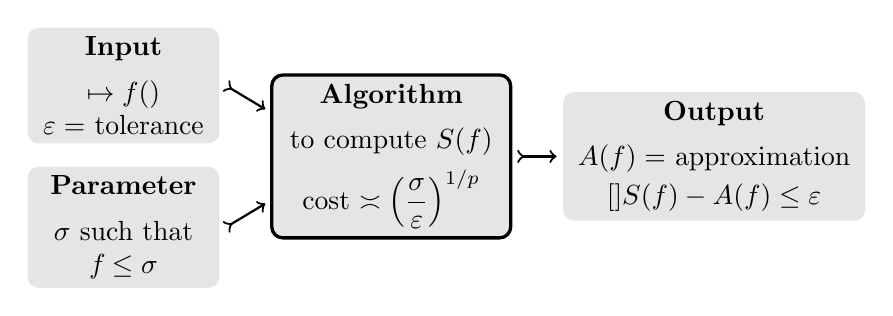
\begin{tikzpicture}
[auto,
block/.style ={rectangle, very thick, fill=black!10, align=center, rounded corners, minimum height=3em}]
%[auto,
%block/.style ={rectangle, very thick, fill=red!15, align=center, rounded corners, minimum height=3em}]
\draw (1.1,0.9) node[block, text width=2.2cm] {\parbox{2.2cm}{\centering {\bf Input}\\[1ex]
$\vx \mapsto f(\vx)$\\ 
$\varepsilon = $ tolerance}};
\draw (1.1,-0.9) node[block, text width=2.2cm] {\parbox{2.2cm}{\centering {\bf Parameter}\\[1ex]
$\sigma$ such that $\Fnorm{f} \le \sigma$}};
\draw (4.5,0) node[block, draw=black, text width=2.8cm] {\parbox{2.8cm}{\centering{\bf Algorithm}\\[1ex] to compute $S(f)$ \\[1ex]
%\draw (4.5,0) node[block, draw=red, text width=2.8cm] {\parbox{2.8cm}{\centering{\bf Algorithm}\\[1ex] to compute $S(f)$ \\[1ex]
cost $\displaystyle \asymp \left(\frac{\sigma}{\varepsilon}\right)^{1/p}$}};
\draw (8.6,0) node[block, text width=3.6cm] {\parbox{3.6cm}{\centering {\bf Output}\\[1ex] $A(f) = $ approximation \\[0.5ex] $\norm[\ch]{S(f)-A(f)} \le \varepsilon$}};
\draw [>->,thick] (2.4,0.9) -- (2.9,0.6);
\draw [>->,thick] (2.4,-0.9) -- (2.9,-0.6);
\draw [>->,thick] (6.1,0) -- (6.6,0);
\end{tikzpicture}
\caption{Diagram of a guaranteed, non-adaptive algorithm. \label{fig:NonadaptAlgo}}
\end{figure}

The semi-norm $\Fnorm{f}$ may be thought of as the \emph{difficulty of the problem}.  In practice, it is difficult to know a priori the maximum possible value of $\Fnorm{f}$, so having to determine $\sigma$ in advance is a practical drawback of the algorithm in Figure \ref{fig:NonadaptAlgo}.  Moreover, since the computational cost of this algorithm depends on $\sigma$, not $\Fnorm{f}$, the cost does not decrease if $\Fnorm{f}$ is drastically smaller than $\sigma$.  

Adaptive algorithms use function data to try to bound $\Fnorm{f}$ or to estimate $\norm[\ch]{S(f)-A_n(f)}$, so that their computational cost can be adjusted accordingly. Unfortunately, the bounds on $\Fnorm{f}$ and the estimates of $\norm[\ch]{S(f)-A_n(f)}$ are typically heuristic or valid only in the limit of $n \to \infty$.  Thus, these approaches are not guaranteed to provide the answer to within the specified error tolerance for finite $n$.  

Here we show how to construct a \emph{rigorous} upper bound on $\Fnorm{f}$ from data, which then leads to a guaranteed automatic and adaptive algorithm.  The key idea is to consider functions lying in a \emph{cone} instead of a ball.  A cone is a set with the property that any positive multiple of an element in the set is also in the set.  Let $\cg$ be some superspace of $\cf$ with a weaker semi-norm, and define the cone
\begin{equation} \label{conedef}
\cc_{\tau}=\{f \in \cf : \Fnorm{f} \le \tau \Gnorm{f} \}.
\end{equation}
A function inside the cone may have a large semi-norm, but its $\cg$-semi-norm can be estimated with reasonable effort.  Our approach to obtaining a reliable approximation to the true solution is sketched here:

\begin{itemize}
\item Since the $\cg$-semi-norm is weaker than the $\cf$-semi-norm, it can be approximated by some algorithm $G_n(f)$, with $\Gnorm{f}-G(f) \le h_+(n)\Fnorm{f}$ for some known $h_+(n)$ that vanishes as $n \to \infty$.  One chooses a sample size $n_G$ such that $h_+(n_G) \le 1/\tau$.

\item The definition of the cone in \eqref{conedef} implies that 
\[
\Gnorm{f} \le G_{n_G}(f)+ h_+(n_G)\Fnorm{f} \le G_{n_G}(f)+ \tau h_+(n_G)\Gnorm{f},
\]
and so $\Gnorm{f} \le G_{n_G}(f)/(1 - \tau h_+(n_G))$.

\item Applying the cone condition again leads to an upper bound on the $\cf$-semi-norm, namely,  $\Fnorm{f} \le \tau G_{n_G}(f)/(1 - \tau h_+(n_G))$.

\item This data-driven upper bound on $\Fnorm{f}$ can be used with \eqref{costupbd} to guarantee that the error tolerance will be met using $A_n$ with
\[
n=\cost(A_n)\le \left \lceil\left(\frac{ C_{\up}\tau G_{n_G}(f)}{\varepsilon(1 - \tau h_+(n_G))}\right)^{1/p} \right \rceil.
\]

\item If, as often is the case, $G_{n_G}(f)$ does not overestimate the $\cg$-semi-norm of $f$, one can be assured that the above criterion will be met for 
\[
n=\cost(A_n)\le \left \lceil\left(\frac{ C_{\up}\tau \Gnorm{f})}{\varepsilon(1 - \tau h_+(n_G))}\right)^{1/p} \right \rceil.
\]
Given that $\Fnorm{f} = \tau \Gnorm{f}$ for some $f$, the cost of this algorithm as $\varepsilon \to 0$ is asymptotically the same as if one did know $\Fnorm{f}$ in advance.

\item On top of the above analysis, we allow for a maximum computational cost budget, $N_{\max}$, that allows the user to specify how long he or she is willing to wait for an answer.

\end{itemize} 
Figure \ref{fig:AdaptAlgo} is a diagram of the automatic algorithm just outlined.

\begin{figure}[h]
\centering
\begin{tikzpicture}
[auto,
block/.style ={rectangle, very thick, fill=black!10, align=center, rounded corners, minimum height=3em}]
%[auto,
%block/.style ={rectangle, very thick, fill=red!15, align=center, rounded corners, minimum height=3em}]
\draw (1.2,0.9) node[block, text width=2.4cm] {\parbox{2.4cm}{\centering{\bf Input}\\[0.5ex] 
$\vx \mapsto f(\vx)$\\ 
$\varepsilon = $ tolerance}};
\draw (1.2,-1.2) node[block, text width=2.4cm] {\parbox{2.4cm}{\centering{\bf Parameters}\\[0.5ex] 
$\tau$ such that $\Fnorm{f} \le \tau\Gnorm{f}$ \\[0.5ex] $N_{\max} = $ cost budget}};
\draw (4.9,0) node[block, draw=black, text width=3.2cm] {\parbox{3.2cm}{\centering{\bf Algorithm}\\[0.5ex] to compute $S(f)$ \\[1ex]
%\draw (5.1,0) node[block, draw=red, text width=3.2cm] {\parbox{3.2cm}{\centering{\bf Algorithm}\\[1ex] to compute $S(f)$ \\[1ex]
cost $\displaystyle \asymp \left(\frac{\tau\Gnorm{f}}{\varepsilon}\right)^{1/p}$ }};
\draw (9.2,0) node[block, text width=3.6cm] {\parbox{3.6cm}{\centering{\bf Output}\\[0.5ex] $A(f) = $ approximation \\[0.5ex] $\norm[\ch]{S(f)-A(f)} \le \varepsilon$}};
\draw [>->,thick] (2.6,0.9) -- (3.1,0.6);
\draw [>->,thick] (2.6,-0.9) -- (3.1,-0.6);
%\draw [>->,thick] (2.6,0) -- (3.1,0);
\draw [>->,thick] (6.7,0) -- (7.2,0);
\end{tikzpicture}
\caption{Diagram of a guaranteed, adaptive, automatic algorithm. \label{fig:AdaptAlgo}}
\end{figure}

Section \ref{integsec} presents a concrete example of this approach for the problem of computing the integral $\int_0^1 f(x) \, \dif x$ for all integrands whose second derivatives are absolutely integrable, i.e., $\Fnorm{f}=\norm[1]{f''}$. The trapezoidal rule based on $n$ function values, i.e., $n-1$ trapezoids, computes an approximation with error no greater than $\varepsilon$ using $2+ \sqrt{\norm[1]{f''}/(8\varepsilon)}$ function values.  However, except for relatively simple integrands, a bound on $\norm[1]{f''}$ is unknown in practice.  

Following the procedure outlined above we choose the weaker semi-norm as $\Gnorm{f} = \norm[1]{f'-f(1)+f(0)}$.  This semi-norm may be estimated by an algorithm $G_n$ that takes the $\cg$-semi-norm of the piecewise linear spline for $f$.  The error for $G_n(f)$ is bounded by $\norm[1]{f''}/(2n-2)$.  Fixing the parameter $\tau > 1$, and assuming that $\norm[1]{f''} \le \tau \norm[1]{f'-f(1)+f(0)}$  (the cone condition), then the reliable numerical upper bound on $\norm[1]{f'}$ can be used to obtain an upper bound for $\norm[1]{f''}$.   
This leads to a guaranteed, automatic (adaptive) algorithm for approximating the integral to the desired accuracy with a computational cost that is no greater than $4+ \tau + \sqrt{\tau \norm[1]{f'-f(1)+f(0)}/(2\varepsilon)}$ (Theorem \ref{multistageintegthm}), where $\norm[1]{f'-f(1)+f(0)}$ is unknown a priori.  Here $\tau$ represents a minimum sample size, and $1/\tau$ represents a length scale of for possible spikes that one wishes to integrate accurately.

There are limited theoretical results providing conditions under which adaption is useful.  Novak \cite{Nov96a} shows the advantage of adaption in for some problems in the average case and randomized settings.  Plaskota and Wasilkowski \cite{PlaWas05a,PlaEtal08a} demonstrate the advantage of adaption for integrating or approximating functions with singularities. By contrast, here we consider the deterministic setting, and we are not concerned with functions with singularities.

This article starts with the general setting and then moves to two concrete cases.  Section \ref{probdefsec} lays out the problems to be solved.  Section \ref{NonAdaptsec} defines non-adaptive algorithms, their costs, and the complexities of numerical problems for which non-adaptive algorithms are suited.  The algorithm diagrammed in Figure \ref{fig:NonadaptAlgo} is essentially this kind of algorithm.  Non-adaptive algorithms are the building blocks for adaptive algorithms.  Adaptive algorithms, their costs, and the complexity of problems defined on cones of functions are introduced in Section \ref{AutoAlgsec}.  The maximum and minimum costs of algorithms are defined in terms of the unknown, but estimated, $\cg$-semi-norm of the input function.  The problem definition here allows for a maximum computational cost budget to be imposed so that one never needs to wait an arbitrarily large time for the answer.  

Sections \ref{genthmsec} and \ref{LowBoundSec} describes the automatic algorithms in detail and provides proofs of their success for cones of input functions.  Although the long term goal of this research is to construct good locally adaptive algorithms, where the sampling density varies according to the function data, here we present only globally adaptive algorithms, where the sampling density is constant, but the number of samples is determined adaptively.  In particular, the following results are presented:
\begin{itemize}

\item Algorithm \ref{twostagedetalgo} is a two stage algorithm: $\Gnorm{f}$ is bounded above once, and  this bound is used to determine the additional computational cost, $n$, such that $A_n(f)$ achieves the desired accuracy. Algorithm \ref{multistagealgo} is a multi-stage algorithm, where the algorithm, $G_n$, used to bound $\Gnorm{f}$, and the algorithm, $A_n$, used to approximate $S(f)$, are based on the same data. Moreover, these are embedded algorithms whose costs increase progressively according to some sequence $n_1, n_2, \ldots$.  Once the number of samples is sufficiently large so that $g_{n_i}(f)$ is small enough, the algorithm terminates.

\item Theorems \ref{TwoStageDetermThm} and \ref{MultiStageThm} in Section \ref{genthmsec} prove that Algorithms \ref{twostagedetalgo} and \ref{multistagealgo}, respectively, are guaranteed to produce answers to within the desired error tolerance, provided that they do not exceed the maximum cost budget.  These theorems also demonstrate that the computational costs of these algorithms do not exceed the costs of algorithms that know $\Fnorm{f}$ or $\Gnorm{f}$ a priori.

\item Theorem \ref{complowbd} in Section \ref{LowBoundSec} provides lower bounds on the computational complexity of the problems defined on cones of input functions by constructing fooling functions.  Corollary \ref{optimcor} shows that Algorithms \ref{twostagedetalgo} and \ref{multistagealgo} are optimal if the non-adaptive algorithms on which they are based are optimal for problems defined on balls of input functions.

\end{itemize}

Section \ref{integsec} illustrates the general results in Sections \ref{genthmsec} and \ref{LowBoundSec} for the univariate integration problem.  An explicit automatic algorithm based on the trapezoidal rule is presented and its success and optimality are proved in Theorem \ref{multistageintegthm}.  Section \ref{approxsec}  considers function approximation with analogous results.  Common concerns about automatic and adaptive algorithms are answered in Section \ref{overcomesec}. The article ends with several suggestions for future work.

\section{General Problem Definition} \label{probdefsec}

\subsection{Problems and Algorithms} The function approximation, integration, or other problem to be solved is defined by a \emph{solution operator} $S:\cf \to \ch$, where $\cf$ is a Banach space of possible input functions defined on $\cx$ with semi-norm $\Fnorm{\cdot}$, and $\ch$ is some other Banach space of possible outputs or solutions with norm $\norm[\ch]{\cdot}$. The solution operator is assumed to have a scale property, i.e., 
\[
S(cf) = cS(f) \qquad \forall c\ge 0.
\]
Examples include the following:
\begin{align*}
\text{Integration:} \quad & S(f) = \int_{\cx} f(\vx) \, \rho(\vx) \, \dif \vx, \quad \rho \text{ is fixed,}\\
\text{Function Recovery:} \quad & S(f) = f, \\
\text{Poisson's Equation:} \quad & S(f) = u, \quad \text{where } \begin{array}{c} -\Delta u(\vx) = f(\vx), \ \vx \in \cx, \\ u(\vx)=0 \ \forall \vx \in \partial \cx, \text{ and}\end{array} \\
\text{Optimization:} \quad & S(f) = \min_{\vx \in \cx} f(\vx).
\end{align*}
The first three examples above are linear problems, but the last example is a nonlinear problem, which nevertheless also has the scale property.

The goal is to find an algorithm $A:\cf \to \ch$ for which $S(f) \approx A(f)$. Following the definition of algorithms described in \cite[Section 3.2]{TraWasWoz88}, the algorithm takes the form of some function of data derived from the input function:
\begin{equation}
\label{algoform}
A(f) =  \phi(\vL(f)), \quad \vL(f) = \left(L_1(f), \ldots, L_m(f)\right) \qquad \forall f \in \cf.
\end{equation}
Here the $L_i \in \Lambda$ are real-valued functions defined on $\cf$ with the following scale property:
\begin{equation}
\label{dataassump}
L(cf) = cL(f) \qquad \forall f \in \cf, \ c \in \reals, \ L \in \Lambda.
\end{equation}
One popular choice for $\Lambda$ is the set of all function values, $\Lambda^{\std}$, i.e., $L_i(f) = f(\vx_i)$ for some $\vx_i \in \cx$.  Another common choice is the set of all bounded linear functionals, $\Lambda^{\lin}$.  In general, $m$ may depend on $f$ and the choice of $L_i$ may depend on $L_1(f), \ldots, L_{i-1}(f)$.  In this article, all algorithms are assumed to be deterministic.  There is no random element.

\subsection{Non-Adaptive Algorithms} \label{NonAdaptsec}

The set $\ca_{\fix}(\cf,\ch,S,\Lambda)$ contains non-adaptive algorithms, i.e., those algorithms for which the choice of the $L_i$ and the number of function data used both independent of the input function.  Furthermore, any $A \in \ca_{\fix}(\cf,\ch,S,\Lambda)$ is assumed to satisfy the following scale properties:
\begin{equation}
\label{algoscale}
\vL(cf) = c \vL(f), \quad 
\phi(c\vy) = c\phi(\vy), \quad A(cf) = cA(f) \qquad \forall c \ge 0, \ \vy \in \reals^m.
\end{equation}

The cost of a non-adaptive algorithm, $A \in  \ca_{\fix}(\cf,\ch,S,\Lambda)$, is fixed and is defined as the sum of the costs of all the function data:
\begin{equation} \label{costfix}
\cost(A) = \$(\vL) = \$(L_1) + \cdots +\$(L_m),
\end{equation}
where $\$:\Lambda \to [1,\infty)$, and $\$(L)$ is the cost of acquiring the datum $L(f)$. The cost of $L$ may be the same for all $L \in \Lambda$, e.g, $\$(L)=1$.  Alternatively, the cost might vary with the choice of $L$.  For example, if $f$ is a function of the infinite sequence of real numbers, $(x_1, x_2, \ldots)$, the cost of evaluating the function with arbitrary values of the first $d$ coordinates, $L(f)=f(x_1, \ldots, x_d, 0, 0, \ldots)$, might be $d$.  This cost model has been used by \cite{HicMGRitNiu09a,KuoEtal10a,NiuHic09a,NiuHic09b,PlaWas11a} for integration problems and \cite{Was13a,WasWoz11a,WasWoz11b} for function approximation problems.

It is assumed that any non-adaptive algorithm $A  \in \ca_{\fix}(\cf,\ch,S,\Lambda)$ is exact for all inputs with zero semi-norm, i.e., $S(f)=A(f)$, for all $f$ with $\Fnorm{f}=0$.  The error of a non-adaptive algorithm is defined  as
\begin{equation} \label{errdefworst}
\err(A,\cf,\ch,S)= \sup_{\substack{f \in \cf\\ \Fnorm{f} \ne 0}}  \frac{\norm[\ch]{S(f) -  A(f)}}{\Fnorm{f}}.
\end{equation}
When the problem has real-valued solutions, i.e., $\ch=\reals$, one may also define a one sided error criterion:
\begin{equation}\label{errpmdefworst}
\err_{\pm}(A,\cf,\reals,S) = \sup_{\substack{f \in \cf\\ \Fnorm{f} \ne 0}}  \frac{\pm[S(f) -  A(f)]}{\Fnorm{f}} . 
\end{equation}

The above error criteria are normalized, meaning that the absolute error, $\norm[\ch]{S(f) -  A(f)}$, is measured with respect to the $\cf$-semi-norm of the input function. The complexity of a problem for this set of algorithms, $\ca_{\fix}(\cf,\ch,S,\Lambda)$, is defined as the cost of the cheapest algorithm that satisfies the specified error tolerance, $\varepsilon$:
\begin{multline} \label{fixcostcomplex}
\comp(\varepsilon,\ca_{\fix}(\cf,\ch,S,\Lambda)) \\
= \inf\left\{\cost(A) : \err(A,\cf,\ch,S) \le \varepsilon, \ A \in \ca_{\fix}(\cf,\ch,S,\Lambda) \right \}.
\end{multline}
Here the infimum of an empty set is defined to be $\infty$.  So, to guarantee that $\norm[\ch]{S(f) -  A(f)} \le \varepsilon$, one needs an algorithm with a cost of at least 
\[
\comp(\varepsilon/\Fnorm{f},\ca_{\fix}(\cf,\ch,S,\Lambda)).
\]
This cost is non-increasing as either $\varepsilon$ decreases or $\Fnorm{f}$ increases.

Suppose that there is a sequence of nonadaptive algorithms indexed by their cost, and which converge to the true answer:
\begin{subequations} \label{algseqdef}
\begin{gather} 
\{A_n\}_{n \in \ci}, \qquad A_n  \in \ca_{\fix}(\cf,\ch,S,\Lambda), \\
\lim_{\substack{n \to \infty\\ n \in \ci}} \err(A_n,\cf,\ch,S) = 0, \qquad \cost(A_n) = n,  
\end{gather}
\end{subequations}
where the countable, non-negative-valued index set, 
\begin{equation} \label{indexdef}
\ci=\{n_1, n_2, \ldots\} \quad \text{with } n_i < n_{i+1}, \quad \text{satisfies } \sup_i \frac{n_{i+1}}{n_i} <\infty. 
\end{equation} 
This sequence of algorithms is called \emph{optimal} for the problem $(\cf,\ch,S,\Lambda)$ if it essentially tracks the minimum cost algorithms, namely,
\begin{equation} \label{nearoptdef}
\sup_{0 < \varepsilon \le 1} \frac{\min\{n \in \ci : \err(A_n,\cf,\ch,S) \le \varepsilon\}} {\comp(\varepsilon,\ca_{\fix}(\cf,\ch,S,\Lambda))} <\infty.
\end{equation}

\subsection{Automatic, Adaptive Algorithms} \label{AutoAlgsec}

Non-adaptive algorithms, $A \in \ca_{\fix}(\cf,\ch,S,\Lambda)$ need an upper bound on $\Fnorm{f}$ to guarantee that they meet the prescribed error tolerance for the input function $f$.  Adaptive algorithms attempt to estimate $\Fnorm{f}$ and then determine the number of function data needed to meet the error tolerance.  The definitions of automatic, adaptive algorithms given in this subsection, differ somewhat from the definitions of non-adaptive algorithms in the previous subsection.  However, automatic algorithms use non-adaptive algorithms as building blocks.

Practical automatic algorithms in $\ca(\cf,\ch,S,\Lambda)$ take the form of ordered pairs of functions
\[
(A,W): \cf \times (0,\infty)\times [1,\infty] \to \ch \times \{\text{false},\text{true}\},
\]
for which one hopes that $S(f) \approx A(f;\varepsilon,N_{\max})$.  Here $\varepsilon \in (0,\infty)$ is a user-supplied error tolerance, $N_{\max} \in [1,\infty]$ is a user-supplied maximum cost budget, and $W(f;\varepsilon,N_{\max})$ is a Boolean warning flag that is false if the algorithm completed its calculations without attempting to exceed the cost budget, and is true otherwise.  

As in \eqref{algoform}, the algorithm is some function of function data: $A(f;\varepsilon,N_{\max}) = \phi\left(\vL(f);\varepsilon,N_{\max}\right)$.
Now, however, the algorithm is allowed to be adaptive. The choice of $L_2$ may depend on the value of $L_1(f)$, the choice of $L_3$ may depend on $L_1(f)$ and $L_2(f)$, etc.  The number of function data used by the algorithm, $m$, may also be determined adaptively. The choice of how many and which function data to use depends on $\varepsilon$ and $N_{\max}$.  Thus, $\vL(c\vy)$ might not equal $c\vL(\vy)$ since the length of the information vector depends on the data recorded.  The goal of the algorithm is to make $\norm[\ch]{S(f) - A(f;\varepsilon,N_{\max})} \le \varepsilon$, but this is not a requirement of the definition.

The cost of the algorithm for a specified input function is defined analogously to \eqref{costfix} as the sum of the costs of all function data.
\[
\cost(A,f;\varepsilon,N_{\max}) = \$(\vL) = \$(L_1) + \cdots +\$(L_m).
\]
Because of the potentially adaptive nature of the algorithm, namely that $m$ may depend on $f$, it follows that the cost may depend on $f$ as well as $A$. The input parameter $N_{\max}$ tells the algorithm to ensure that $\cost(A,f;\varepsilon,N_{\max}) \le N_{\max}$ for all $f$ and $\varepsilon$.  This is a practical consideration since the user does not want to wait indefinitely for an answer. 

The automatic, adaptive algorithms developed here are valid for subsets of $\cf$ that may be unbounded, e.g., cones of functions, $\cc_{\tau}$, as described in Section \ref{conesubsec}, or their subsets, $\cn$.  The design of the algorithm depends on the definition of $\cn$.  The computational cost of the adaptive algorithm for $f$ in $\cn$ may be quite large or even arbitrarily large, depending on the $\cf$-semi-norm of $f$.  We want to find upper and lower bounds on the cost of the algorithm that take into account more information about $f$, say that it lies in some ball. However, the definition of the ball is not used by the algorithm, but only as a device to measure computational cost. Let $\cb_{\sigma}$ denote the $\cf$-semi-norm ball defined in \eqref{balldef}.  For automatic algorithms defined with respect to some set of functions $\cn \subset \cf$, we define the \emph{maximum} cost of the algorithm relative to $\cb_{\sigma}$ as follows:
\begin{equation*}
\maxcost(A,\cn,\varepsilon,N_{\max},\cb_{\sigma})
= \sup \{ \cost(A,f;\varepsilon,N_{\max}) : f \in \cn \cap \cb_{\sigma} \} .
\end{equation*}
Here the set $\cn$ is allowed to depend on the algorithm inputs, $\varepsilon$ and $N_{\max}$, but not on $\sigma$.  Again we stress that $A$ knows $\cn$ but not $\cb_\sigma$.

One would prefer an algorithm where the costs for different input functions with the same size or norm to be similar.  To make this precise we define the  \emph{minimum} cost:
\begin{equation*}
\mincost(A,\cn,\varepsilon,N_{\max},\cb_\sigma)
= \inf \left \{ \cost(A,f;\varepsilon,N_{\max}) : f \in \cn\setminus \bigcup_{\sigma'<\sigma}\cb_{\sigma'} \right\} .
\end{equation*}
An algorithm is said to have \emph{stable computational cost} if 
\begin{equation*}
\sup_{\substack{\varepsilon, \sigma > 0\\ 0 < \varepsilon < \sigma}} \frac{\maxcost(A,\cn,\varepsilon,N_{\max},\cb_\sigma)}{\mincost(A,\cn,\varepsilon,N_{\max},\cb_\sigma)} < \infty.
\end{equation*}

For automatic algorithms, returning an approximation with the desired error is not enough.  One also wants the algorithm to be confident that the answer is correct.  An  algorithm  $(A,W) \in \ca(\cn,\ch,S,\Lambda)$, is deemed successful provided that it meets the prescribed error tolerance and does not raise the warning flag.  Specifically, success is defined as
\begin{multline*}
\success(A,W,\cn,\varepsilon,N_{\max}) \\
= \begin{cases} \text{true} & \text{if } \displaystyle \norm[\ch]{S(f)-A(f;\varepsilon,N_{\max})} \le \varepsilon \ \& \ W(f;\varepsilon,N_{\max})=\text{false} \quad \forall  f \in \cn, \\
\displaystyle \text{false} & \text{otherwise}.
\end{cases}
\end{multline*}
The above are absolute error criteria for success.  One might also define relative error criteria instead, but finding successful algorithms for relative error is a non-trivial exercise and will be considered in future work.

The complexity of a problem is defined as the maximum cost of the cheapest successful algorithm for input functions with $\cg$-semi-norm no greater than $\sigma$:
\begin{multline} \label{complexdef}
\comp(\varepsilon,\ca(\cn,\ch,S,\Lambda),N_{\max},\sigma) \\
 = \inf\left\{\maxcost(A,\cn,\varepsilon,N_{\max},\sigma) : \success(A,W,\cn,\varepsilon,N_{\max}) = \text{true}, \right .\\
\left.  (A,W) \in \ca(\cn,\ch,S,\Lambda) \right \}.
\end{multline}
Here the infimum of an empty set is defined to be $\infty$.  The optimality of adaptive algorithms is defined analogously to \eqref{nearoptdef}.

The set of non-adaptive algorithms, $\ca_{\fix}(\cf,\ch,S,\Lambda)$, defined in the previous subsection is a subset of the automatic algorithms $\ca(\cf,\ch,S,\Lambda)$.  Algorithms in $\ca_{\fix}(\cf,\ch,S,\Lambda)$ are not affected by the error tolerance $\varepsilon$ and do not recognize a cost budget $N_{\max}$.  Moreover, the warning flag for an algorithm in $\ca_{\fix}(\cf,\ch,S,\Lambda)$ is always returned as false.  Whereas the non-adaptive algorithms are inherently impractical by themselves, they are vital components of automatic, adaptive algorithms.

\subsection{Cones of Functions} \label{conesubsec} All algorithms can be fooled by some input functions, even if these functions are sufficiently smooth.  An algorithm and error analysis such as that in \eqref{traditionerr} rules out fooling functions with large error by restricting the size of  $\Fnorm{f}$.  

It is often difficult to know how large $\Fnorm{f}$ is a priori and so practical automatic algorithms try to bound it.  The framework described here rules out fooling functions whose $\cf$-semi-norms cannot be reliably bounded above.  This is done by considering $\cg$, a superspace of $\cf$, with its own semi-norm $\Gnorm{\cdot}$.   The semi-norm $\Gnorm{\cdot}$ is considered to be weaker than $\Fnorm{\cdot}$ in the following sense:
\begin{subequations} \label{FGcond}
\begin{equation} \label{Fspacecondstrong}
\tau_{\min} \Gnorm{f} \le \Fnorm{f} \qquad \forall f \in \cf,
\end{equation}
where $\tau_{\min}$ is some \emph{positive} constant.  Here, the subspace of functions in $\cg$ with vanishing $\cg$-semi-norm, is assumed to be a finite dimensional subspace of $\cf$ as well, and by the above condition must be contain the subspace of of functions with vanishing $\cf$-semi-norm, i.e.,
\begin{equation} \label{nullspacecond}
\cf_0:=\{f \in \cf : \Fnorm{f}=0\} \subseteq \cg_0:=\{f \in \cg : \Gnorm{f}=0\} \subset \cf.
\end{equation}
\end{subequations}

Given $\tau>0$, let $\cc_{\tau} \subset \cf$ denote a \emph{cone} of functions whose $\cf$-semi-norms are no greater than $\tau$ times their $\cg$-semi-norms, as defined in \eqref{conedef}. This means that 
\begin{equation} \label{twosidedFGbound}
\tau_{\min} \Gnorm{f} \le \Fnorm{f} \le \tau \Gnorm{f} \qquad \forall f \in \cc_{\tau}
\end{equation} 
Note that one must choose $\tau \ge \tau_{\min}$ for $\cc_{\tau}$ to contain functions outside $\cg_0$.  Moreover, $\cf_0= \cg_0 \cap \cc_{\tau}$.

For any $f \in \cc_{\tau}$ both $\Fnorm{f}$ and $\Gnorm{f}$ must be finite, but they can be arbitrarily large.  There is no need to assume an upper bound on their sizes, but it is possible to obtain reliable upper bounds for both $\Fnorm{f}$ and $\Gnorm{f}$ by sampling $f$.  This argument appears to be circular, but is in fact valid.  An upper bound on $\Gnorm{f}$ for $f \in \cc_{\tau}$ can be computed in terms of the data $\vL(f)=(L_1(f), \ldots, L_m(f))$ because $\Fnorm{\cdot}$ is a stronger semi-norm than $\Gnorm{\cdot}$ in the sense of \eqref{Fspacecondstrong}, and because $\Fnorm{f}$ is no larger than a multiple of $\Gnorm{f}$ (see Lemma \ref{Gnormlem} below). This upper bound on $\Gnorm{f}$ then automatically implies an upper bound on $\Fnorm{f}$ from the definition of the cone. These reliable bounds on both $\Fnorm{f}$ and $\Gnorm{f}$ may be used to obtain a bound on the error of the algorithm for estimating $S(f)$  (see Theorem \ref{TwoStageDetermThm} below).

\subsection{Results that We Prove}  The previous subsections define the problem to be approximated and the notation describing the difficulty of the problem and the efficiency of the algorithms.  This subsection summarizes the results that are proved in general in the next two sections and illustrated for specific cases in the Sections \ref{integsec} and \ref{approxsec}.

\begin{enumerate}

\renewcommand{\labelenumi}{\roman{enumi}.}

\item \emph{Upper bound on the complexity.}
Theorems \ref{TwoStageDetermThm}, \ref{MultiStageThm}, \ref{multistageintegthm}, and \ref{multistageappxthm} provide upper bounds on the complexity of solving the problem, $\comp(\cn,\varepsilon,N_{\max},\sigma,\Lambda)$, in terms of some function of $\varepsilon/\sigma$ and for the set $\cn \subset \cc_{\tau}$.

\item \emph{An algorithm that achieves the upper bound.}  Algorithms \ref{twostagedetalgo} and \ref{multistagealgo} provide explicit, constructive frameworks for two kinds of successful algorithms, $(A,W) \in \ca(\cn,\ch,S,\Lambda)$, that achieve these upper bounds.  Algorithms \ref{multistageintegalgo} and \ref{multistageapproalgo} provide concrete cases.

\item \emph{Penalty for not knowing the $\cf$- and $\cg$-semi-norms of $f$.} The optimal successful algorithm must find an upper bound on $\Fnorm{f}$ or $\Gnorm{f}$ rather than assuming such an upper bound.  One hopes that the extra cost relative to the situation of knowing a priori bounds on these semi-norms is not too great.  Positive results are given in Theorems  \ref{TwoStageDetermThm}, \ref{MultiStageThm}, \ref{multistageintegthm}, and \ref{multistageappxthm}.

\item \emph{Stable Computational Cost.}  The cost of solving the problem for a given tolerance, $\varepsilon$, and an input function with a given value of the $\cg$-semi-norm, $\Gnorm{f}$, varies somewhat depending on the particulars of $f$.  However, we do not want too much variation.  Theorems  \ref{TwoStageDetermThm}, \ref{MultiStageThm}, \ref{multistageintegthm}, and \ref{multistageappxthm} provide positive results on the stability of the computational cost.

\item \emph{Lower bound on the complexity and optimality of algorithms.}  Lower bounds on the complexity of the problem, i.e., the problem's difficulty, are given in Theorem \ref{complowbd}.  Conditions under which Algorithms \ref{twostagedetalgo} and \ref{multistagealgo} attain these lower bounds are given in Corollary \ref{optimcor}.  Specific examples for univariate integration and function recovery are given in Theorems \ref{complowbdinteg} and \ref{complowbdappr}.

\end{enumerate}

\section{General Algorithms and Upper Bounds on the Complexity} \label{genthmsec}

This section provides rather general theorems about the complexity of automatic algorithms.  In some sense, these theorems are a road map because their assumptions are non-trivial and require effort to verify for specific problems of interest.  On the other hand, the assumptions are reasonable as is demonstrated in Sections \ref{integsec} and \ref{approxsec} where concrete cases are are discussed.  

\subsection{Bounding the $\cg$-Semi-Norm} \label{Galgosec}

As mentioned in Section \ref{conesubsec} automatic algorithms require reliable upper bounds on $\Gnorm{f}$ for all $f$ in the cone $\cc_{\tau}$. These can be obtained using any non-adaptive algorithm $G_n \in \ca_{\fix}(\cf,\reals_+,\Gnorm{\cdot},\Lambda)$ for approximating $\Gnorm{f}$ for $f \in \cf$ and having cost $n$, provided that one has explicit upper bounds on the errors of these algorithms as in \eqref{errpmdefworst}.  Namely, $G_n(f)=\Gnorm{f}$ for all $f \in \cf$ with vanishing $\cf$-semi-norm, and there exist non-negative valued, non-increasing functions $h_{\pm}$ such that
\begin{equation} \label{Gerrbds}
\err_{\pm}(G_n,\cf,\reals_{+},\Gnorm{\cdot})
= \sup_{\substack{f \in \cf\\ \Fnorm{f}\ne 0}} \frac{\pm [\Gnorm{f}- G_n(f)]}{\Fnorm{f}} \le h_{ \pm}(n).
\end{equation}
Applying the two-sided bound for the $\cf$- and $\cg$-semi-norms \eqref{twosidedFGbound} and rearranging the above error bound implies that 
\begin{align*} 
G_n(f) &\le \Gnorm{f} + h_{-}(n)\Fnorm{f} \le \begin{cases} [1+ \tau h_{-}(n)]\Gnorm{f} \\
\displaystyle \left [\frac{1}{\tau_{\min}}+h_{-}(n) \right]\Fnorm{f} 
\end{cases} \qquad \forall f \in \cc_{\tau},\\
G_n(f) &\ge \Gnorm{f} - h_{+}(n)\Fnorm{f} \ge \begin{cases} [1 - \tau h_{+}(n)]\Gnorm{f} \\
\displaystyle \left [\frac{1}{\tau}-h_{+}(n) \right]\Fnorm{f} 
\end{cases} \qquad \forall f \in \cc_{\tau}.
\end{align*}

\begin{lem} \label{Gnormlem} Any nonadaptive algorithm $G_n \in \ca_{\fix}(\cf,\reals_+,\Gnorm{\cdot},\Lambda)$ with cost $n=\cost(G_n)$ and two sided error bounds as in \eqref{Gerrbds} yields an approximation to the $\cg$-semi-norm of functions in the cone $\cc_{\tau}$ with the following upper and lower error bounds:
\begin{equation} \label{twosidedGineq}
 \frac{\Fnorm{f}}{\tau \fC_n}  \le \frac{\Gnorm{f}}{\fC_n}  \le G_n(f) \le  \begin{cases} \tfc_n \Gnorm{f} \\[1ex]
\displaystyle \frac{\fc_n \Fnorm{f} }{\tau_{\min}}
\end{cases} \qquad \forall f \in \cc_{\tau},
\end{equation}
where the $\fc_n$, $\tfc_n$, and $\fC_n$ are defined as follows:
\begin{gather} \label{normdeflate}
\fc_n =1 + \tau h_{ -}(n)  \ge \fc_n =1 + \tau_{\min} h_{ -}(n)  \ge 1, \\
\label{norminflate}
\fC_n =\frac{1}{1 - \tau h_{ +}(n)} \ge 1, \qquad \text{assuming } h_{ +}(n) < 1/\tau.
\end{gather}
\end{lem}

\subsection{Two-Stage Automatic Algorithms} \label{twostagesec}

Computing an approximate solution to the problem $S: \cc_{\tau} \to \ch$, e.g., integration or function approximation, depends on non-adaptive algorithms. Suppose that there is a sequence of such of algorithms, $\{A_n\}_{n \in \ci}$, with $A_n  \in \ca_{\fix}(\cg,\ch,S,\Lambda)$, indexed by their cost as defined in \eqref{algseqdef}, and for which upper error bounds are known for both the spaces $\cg$ and $\cf$:
\begin{equation}\label{algseqerrbd}
\err(A_n,\cg,\ch,S) \le \tildeh(n), \qquad \err(A_n,\cf,\ch,S) \le h(n), 
\end{equation}
for some \emph{non-increasing} functions $\tildeh$ and $h$.  The definitions of these errors in \eqref{errdefworst} then implies upper bounds on the error of $A_n(f)$ in terms of the $\cg$-semi-norm of $f$:
\begin{align} \nonumber
\norm[\ch]{S(f) -  A_n(f)} &\le \min(\err(A_n,\cg,\ch,S)\Gnorm{f},\err(A_n,\cf,\ch,S)\Fnorm{f}) \\
\label{Anerrbound}
&\le \min(\tildeh(n),\tau h(n))\Gnorm{f} \qquad \forall f \in \cc_{\tau}.
\end{align}

\begin{algo} \label{twostagedetalgo} {\bf (Automatic, Adaptive, Two-Stage).} Let $\cf$, $\cg$, and $\ch$ be Banach spaces as described above, let $S$ be the solution operator, and let $N_{\max}$ be the maximum cost allowed.  Let $\tau$ be a fixed positive number, and let $G_{n_G} \in \ca_{\fix}(\cf,\reals_+,\Gnorm{\cdot},\Lambda)$ be an algorithm as described in Lemma \ref{Gnormlem} with cost $n_G$ satisfying $h_{+}(n_G) < 1/\tau$.
Moreover, let  $\{A_n\}_{n \in \ci}$, $A_n  \in \ca_{\fix}(\cg,\ch,S,\Lambda)$, be a sequence of algorithms as described in \eqref{algseqdef} and \eqref{algseqerrbd}.  Given  a positive error tolerance, $\varepsilon$, and  an input function $f$, do the following:

\begin{description} 

\item[Stage 1.\ Estimate {$\Gnorm{f}$}.] First compute $G_{n_G}(f)$.  Define the inflation factor $\fC=\fC_{n_G}$ according to \eqref{norminflate}.
Then $\fC G_{n_G}(f)$ provides a reliable upper bound on $\Gnorm{f}$.  

\item [Stage 2.\ Estimate {$S(f)$}.] Choose the sample size need to approximate $S(f)$, namely, $n_A=N_{A}(\varepsilon/(\fC G_{n_G}(f)))$, where 
\begin{equation} \label{Nmindef}
N_{A}(a)= \min\left\{ n \in \ci : \min(\tildeh(n),\tau h(n)) \le a \right\}, \quad a \in (0,\infty).
\end{equation}
If $n_A \le N_{\max}-n_G$, then $S(f)$ may be approximated within the desired error tolerance and within the cost budget.  Set the warning flag, $W$, to false. 
Otherwise, recompute $n_A$ to be within budget, $n_A = \tN_{\max} := \max\{n \in \ci : n\le N_{\max} -  n_G\}$, and set the warning flag, $W$ to true.  Finally, compute $A_{n_A}(f)$ as the approximation to $S(f)$.
\end{description}

Return the result $(A_{n_A}(f),W)$, at a total cost of $n_G+n_A$.  
\end{algo}

The bounds in Lemma \ref{Gnormlem} involving $G_n$ and $\Gnorm{\cdot}$ plus the bounds in \eqref{twosidedFGbound} involving $\Gnorm{\cdot}$ and $\Fnorm{\cdot}$ imply bounds on the desired number of samples in the algorithm above.  Since $N_A$ is a nonincreasing function, it follows that for all $f \in \cc_{\tau}$
\begin{equation*}
N_{A}\left(\frac{\tau \varepsilon}{\Fnorm{f}}\right) \le N_{A}\left(\frac{\varepsilon}{\Gnorm{f}}\right)  \le N_{A}\left(\frac{\varepsilon}{\fC G_{n_G}(f)}\right) \le 
\begin{cases} \displaystyle N_{A}\left(\frac{\varepsilon}{\fC \tfc \Gnorm{f}}\right) \\[1ex]
\displaystyle N_{A}\left(\frac{\tau_{\min} \varepsilon}{\fC \fc \Fnorm{f}}\right)\end{cases}.
\end{equation*}
This means that proposed computational cost to compute $A(f)$ is reasonable, i.e., $N_{A}(\varepsilon/(\fC G_{n_G}(f))) \le \tN_{\max}$ if either of the following conditions holds 
\begin{gather}
\Gnorm{f} \le \varepsilon\tsigma_{\max}, \qquad \tsigma_{\max} := \frac{1}{\fC \tfc \min(\tildeh(\tN_{\max}),\tau h(\tN_{\max}))}, \\
\Fnorm{f} \le \varepsilon\sigma_{\max}, \qquad  \sigma_{\max} := \frac{\tau_{\min}}{\fC \fc \min(\tildeh(\tN_{\max}),\tau h(\tN_{\max}))}.
\end{gather}

\begin{theorem}  \label{TwoStageDetermThm}  Let  $\cf$, $\cg$, $\ch$,  $\tau$, $N_{\max}$, $\tN_{\max}$, $\fC$, and $\varepsilon$ be given as described in Algorithm \ref{twostagedetalgo}, and assume that $\cf$ satisfies \eqref{Fspacecondstrong}.  Let $\fc=\fc_{n_G}$ be defined as in \eqref{normdeflate}.
Let $\cc_\tau$ be the cone of functions defined in \eqref{conedef} whose $\cf$-semi-norms are no larger than $\tau$ times their $\cg$-semi-norms.  Let $\cn$ be the subset of the cone $\cc_\tau$ that lies inside either the $\cg$-semi-norm ball of radius $\varepsilon\tsigma_{\max}$, i.e., $\tcb_{\varepsilon\tsigma_{\max}}$, or the $\cf$-semi-norm ball of radius $\varepsilon\sigma_{\max}$, i.e., $\cb_{\varepsilon\sigma_{\max}}$:  
\begin{equation} \label{nicefdef}
\cn = \cc_\tau \cap (\tcb_{\varepsilon\tsigma_{\max}} \cup \cb_{\varepsilon\sigma_{\max}}).
\end{equation}
Since $\tN_{\max}$ is assumed to be huge, it follows that radii $\tsigma_{\max}$ and $\sigma_{\max}$ are also huge.

Then it follows that Algorithm \ref{twostagedetalgo} is successful for all functions in this set of \emph{nice} functions $\cn$,  i.e.,  $\success(A,W,\cn,\varepsilon,N_{\max}) = \text{true}$.  Moreover, the cost of this algorithm is bounded above and below in terms of the unknown $\cg$- and $\cf$-semi-norms of any input function in $\cn$ as follows:
\begin{subequations}  \label{auto2stagedetcost}
\begin{gather}
n_G+ N_{A}\left(\frac{\varepsilon}{\Gnorm{f}} \right) \le 
\cost(A,f;\varepsilon,N_{\max})
\le n_G+ N_{A}\left(\frac{\varepsilon}{\fC\tfc\Gnorm{f}}\right), \\
n_G+ N_{A}\left(\frac{\tau \varepsilon}{\Fnorm{f}} \right) \le \cost(A,f;\varepsilon,N_{\max})
\le n_G+ N_{A}\left(\frac{\tau_{\min}\varepsilon}{\fC\fc\Fnorm{f}}\right).
\end{gather}
%\begin{gather}
%\maxcost(A,\cn,\varepsilon,N_{\max},\tcb_{\tsigma})
%\le n_G+ N_{A}\left(\frac{\varepsilon}{\fC\tfc\tsigma}\right), \\
%\maxcost(A,\cn,\varepsilon,N_{\max},\cb_{\sigma})
%\le n_G+ N_{A}\left(\frac{\tau_{\min}\varepsilon}{\fC\fc\sigma}\right), \\
%\mincost(A,\cn,\varepsilon,N_{\max},\tcb_{\tsigma})
%\ge n_G+ N_{A}\left(\frac{\varepsilon}{\tsigma} \right),\\
%\mincost(A,\cn,\varepsilon,N_{\max},\cb_{\sigma})
%\ge n_G+ N_{A}\left(\frac{\tau \varepsilon}{\sigma} \right).
%\end{gather}
\end{subequations}
If $N_A(a)$ is polynomial in $a^{-1}$, then this algorithm is computationally stable in the sense that the maximum cost is no greater than some constant times the minimum cost.
\end{theorem}

\begin{proof} The definition of $\fC$ in \eqref{norminflate} implies that the true $\cg$-semi-norm of $f$ is bounded above by $\fC G_{n_G}(f)$ according to Lemma \ref{Gnormlem}.  The upper bound on the error of the sequence of algorithms $\{A_n\}_{n \in \ci}$ in \eqref{Anerrbound} then implies that 
\[
\norm[\ch]{S(f) -  A_n(f)} \le \min(\tildeh(n),\tau h(n)) \fC G_{n_G}(f) \qquad \forall f \in \cc_{\tau}.
\]
This error upper bound may be made no greater than the error tolerance, $\varepsilon$, by choosing the algorithm cost, $n$, to satisfy the condition in Stage 2 of Algorithm \ref{twostagedetalgo}, provided that this can be done within the maximum cost budget.  In this case, the algorithm is successful, as claimed in the theorem.  

The argument preceding the statement of this theorem establishes that Algorithm \ref{twostagedetalgo} does not attempt to overrun the cost budget if $f \in \tcb_{\varepsilon\tsigma_{\max}} \cup \cb_{\varepsilon\sigma_{\max}}$. This argument also establishes the maximum and minimum cost bounds in \eqref{auto2stagedetcost}. 
\end{proof}

There are a several remarks that may facilitate understanding of this result.

\begin{rem} Three main conditions must be checked for this theorem to hold.
\begin{enumerate}
\renewcommand{\labelenumi}{\roman{enumi}.}
\item There must be an algorithm, $G_n$, as described in Section \ref{Galgosec} that approximates the weaker semi-norm,  $\Gnorm{\cdot}$, and its error bound, $h_{\pm}$, as defined in \eqref{Gerrbds} must be known explicitly.
\item There must be a  sequence of nonadaptive algorithms, $\{A_n\}_{n \in \ci}$, as described at the beginning of  Section \ref{twostagesec}, and the error functions $\tildeh$ and $h$, defined in \eqref{algseqerrbd} must be known explicitly.  
\item Condition \eqref{nearoptdef} defining the optimality of $\{A_n\}_{n \in \ci}$ must be satisfied to ensure that there is no significant penalty for not having an a priori upper bound on $\Gnorm{f}$.
\end{enumerate}
Sections \ref{integsec} and \ref{approxsec} provide concrete examples where these conditions are checked.
\end{rem}

\begin{rem} If $\tildeh$ is unknown, then one may take $\tildeh(n)=\infty$, and the algorithm still satisfies the error tolerance with a cost upper bound given in \eqref{auto2stagedetcost}.  The optimality result in \eqref{penalty} then only holds for $\cf$, and not $\cg$.  The analogy holds if $h$ is unknown.  However, at least one of these two functions $\tildeh$ or $h$, must be known for this theorem to be meaningful.
\end{rem}

\begin{rem} The maximum and minimum costs of Algorithm \ref{twostagedetalgo}, as given by \eqref{auto2stagedetcost}, depend on the $\cg$-semi-norm of the input function, $f$.  However, $\Gnorm{f}$ is not an input parameter for the algorithm, but rather is  conservatively estimated by the algorithm.  The number of samples used to obtain the approximation to $S(f)$ is adjusted accordingly based on the estimate of $\Gnorm{f}$.
\end{rem}

\begin{rem}
The definition of the set of algorithms for which the Algorithm \ref{twostagedetalgo} is guaranteed to work, $\cn$, depends somewhat on $\Gnorm{f}$, but only because of the practical constraint of a cost budget of $N_{\max}$.  This dependence disappears if one lifts this constraint by taking $N_{\max} \to \infty$.  The primary constraint determining the success of the algorithm is that $f$ lies in the cone $\cc_{\tau}$.
\end{rem}

\begin{rem} Instead of choosing $\tau$ as an input parameter for Algorithm \ref{twostagedetalgo}, one may alternatively choose the inflation factor $\fC >1$.  This then implies that 
\begin{equation} \label{taufromnC}
\tau = \left(1 - \frac{1}{\fC}\right)\frac{1}{h_{+}(n_G)},
\end{equation}
which is equivalent to \eqref{norminflate}.
\end{rem}

\begin{rem} \label{neccondrem} In some cases it is possible to find a lower bound on the $\cf$-norm of the input function, i.e., there exists an algorithm $F_n$ using the same function values as $G_n$, such that
\[
F_n(f) \le \Fnorm{f} \qquad \forall f \in \cf.
\]
In this case one can use Lemma \ref{Gnormlem} to derive a necessary condition that $f$ is in the cone $\cc_\tau$:
\begin{align}
\nonumber
f \in \cc_\tau 
& \implies F_n(f) \le \Fnorm{f} \le \frac{\tau G_n(f)}{1-\tau h_+(n)}\\
& \implies \tau_{\min,n}:= \frac{F_n(f)}{G_n(f) + h_+(n) F_n(f)} \le \tau.
\label{neccondFn}
\end{align}
For Algorithm \ref{twostagedetalgo} the relevant value of $n$ is $n_G$, whereas for Algorithm \ref{multistagealgo} the relevant value of $n$ is $n_i$.
We stress that this is not a sufficient condition for $f$ to lie in $\cc_{\tau}$, so it is possible to get an incorrect answer from Algorithm \ref{twostagedetalgo} or \ref{multistagealgo} even if the condition above is satisfied.  However, in light of this argument one might modify these algorithms by increasing $\tau$ to, say, $2 \tau_{\min,n}$ in case $\tau_{\min,n}$ ever falls above $\tau$. 
\end{rem}

\begin{rem} It is observed in the examples of Sections \ref{integsec} and \ref{approxsec} that for the sequence of algorithms $\{A_n\}_{n \in \ci}$
\begin{equation} \label{hbest}
\tau h(n) \le \tildeh(n) \quad \forall n \in \ci.
\end{equation}
or equivalently, $\min(\tildeh(n),\tau h(n))=\tau h(n)$.  This then simplifies Algorithm \ref{twostagedetalgo} in the computation of the sample size for $A$ in \eqref{Nmindef} and also in Theorem \ref{TwoStageDetermThm} in the definition of $\cn$ in \eqref{nicefdef} and the upper bound on the cost in \eqref{auto2stagedetcost}. 

A sufficient condition for \eqref{hbest} is
\begin{equation} \label{hbestverb}
h(n) \le \tildeh(n) h_{+}(n) \quad \forall n \in \ci,
\end{equation}
since the Algorithms \ref{twostagedetalgo} and \ref{multistagealgo} both require that $h_{+}(n) < 1/\tau$, and since $h$ is a non-increasing function.   Another 
sufficient condition for \eqref{hbest} is finding some sequence of functions $\{f^*_n \in \cf\}_{n \in \ci}$ with non-zero $\cf$- and $\cg$-semi-norms such that 
\begin{equation} \label{hbestverc}
h(n) \le \frac{\norm[\ch]{S(f^*_n)-A_n(f_n^*)}}{\Gnorm{f_n^*}} \frac{\Gnorm{f^*_n}-G_n(f^*_n)}{\Fnorm{f^*_n}}   \quad \forall n \in \ci,
\end{equation}
since the right hand side above is no greater than the right hand side in \eqref{hbestverb}. An advantage of \eqref{hbestverc} is that it does not require $\tildeh$ to be known explicitly. Finally, suppose that one can construct a sequence of functions $\{f^*_n \in \cf\}_{n \in \ci}$ \emph{with all vanishing data} for both the algorithms $A_n$ and $G_n$ that attains the upper bound on the error of $A_n$ with respect to the $\cf$-semi-norm, i.e.,
\begin{equation} \label{hbestverd}
h(n) = \frac{\norm[\ch]{S(f^*_n)}}{\Fnorm{f^*_n}}   \quad \forall n \in \ci.
\end{equation}
Then this sequence automatically satisfies \eqref{hbestverc}, which then implies \eqref{hbest}.
\end{rem}


\subsection{Automatic Algorithms Based on Embedded Algorithms $\{A_n\}_{n \in \ci}$}

Suppose that the sequence of nonadaptive algorithms, 
\[
\{A_n\}_{n \in \ci} = \{A_{n_1}, A_{n_2}, \ldots \}, 
\]
are \emph{embedded}, i.e., $A_{n_{i+1}}$ uses all of the data used by $A_{n_{i}}$ for $i=1, 2, \ldots$.  An example would be a sequence of composite trapezoidal rules for integration where the number of trapezoids is a power of two. Furthermore, it is supposed that the data used by $G_{n_G}$, the algorithm used to estimate the $\cg$-semi-norm of $f$, is the same data used by $A_{n_1}$, and so $n_1=n_G$.  Then the total cost of Algorithm \ref{twostagedetalgo} can be reduced; it is simply $n_A$, as given in Stage 2, instead of $n_G+n_A$.  Moreover, $\tN_{\max}$ may then be taken to be $N_{\max}$, and the cost bound of the automatic algorithm in \eqref{auto2stagedetcost} does not need the term $n_G$.

Again suppose that $\{A_n\}_{n \in \ci}$, $A_n  \in \ca_{\fix}(\cg,\ch,S,\Lambda)$, consists of algorithms as described in  \eqref{algseqdef} and \eqref{algseqerrbd}, but some of which are embedded in others.  An example would be all possible composite trapezoidal rules for integration that use trapezoids of equal widths.   Moreover, suppose that there exists some fixed $r > 1$ such that for all $n \in \ci$, there exists a $\tn \in \ci$ with $n < \tn \le rn$, such that the data for $A_n$ is embedded in the data for $A_{\tn}$. One may think of $r$ as the minimum cost multiple that one must incur when moving to the next more costly algorithm. For trapezoidal rules, where the cost is the number of trapezoids plus one, one may take $\tn-1=2(n-1)$, so one may choose $r=2$.

Suppose also that there exists a sequence of algorithms for approximating the $\cg$-semi-norm, $\{G_n\}_{n \in \ci}$, $G_n  \in \ca_{\fix}(\cg,\reals_+,\Gnorm{\cdot},\Lambda)$, such that for each $n \in \ci$, $A_n$ and $G_n$ use exactly the same data.
Since $h_{\pm}$ are non-increasing functions, the quantities $\fC_{n}$ and $\fc_n$ do not increase as $n$ increases. These embedded algorithms suggest the following iterative algorithm.

\begin{algo} \label{multistagealgo}  Let the Banach spaces $\cf$, $\cg$, and $\ch$, the solution operator $S$, the maximum cost budget $N_{\max}$, and the positive constant $\tau$ be as described in Algorithm \ref{twostagedetalgo}. Let the sequences of algorithms, $\{A_n\}_{n \in \ci}$ and  $\{G_n\}_{n \in \ci}$ be as described above.  Set $i=1$, and $n_1 = \min\{ n \in \ci : h_+(n) < 1/\tau\}$. For any positive error tolerance $\varepsilon$ and any input function $f$, do the following:
\begin{description}

\item [Stage 1. Estimate $\| f \| _{\cg}$.] Compute $G_{n_i}(f)$ and $\fC_{n_i} \le \infty$ as defined in \eqref{norminflate}.  

\item [Stage 2. Check for Convergence.] Check whether $n_i$ is large enough to satisfy the error tolerance, i.e., 
\begin{equation} \label{multistageconv}
\min(\tildeh(n_i),\tau h(n_i))\fC_{n_i} G_{n_i}(f) \le \varepsilon.
\end{equation}
If this is true, then set $W$ to be false, return $(A_{n_i}(f),W)$ and terminate the algorithm.

\item[Stage 3. Compute $n_{i+1}$.]  Otherwise, if \eqref{multistageconv} fails to hold, compute $\fc_{n_i}$ according to \eqref{normdeflate} using $G_{n_i}$. Choose $n_{i+1}$ as the smallest number exceeding $n_i$ and not less than $N_{A}(\varepsilon \fc_{n_i}/G_{n_i}(f))$ such that $A_{n_{i}}$ is embedded in $A_{n_{i+1}}$. If $n_{i+1} \le N_{\max}$, increment $i$ by $1$, and return to Stage 1.  

Otherwise, if $n_{i+1} > N_{\max}$, choose $n_{i+1}$ to be the largest number not exceeding $N_{\max}$ such that $A_{n_{i}}$ is embedded in $A_{n_{i+1}}$, and set $W$ to be true. Return $(A_{n_{i+1}}(f),W)$ and terminate the algorithm.
\end{description}  
\end{algo}

This iterative algorithm is guaranteed to converge also, and its cost can be bounded.  The following theorem is analogous to Theorem \ref{TwoStageDetermThm}.

\begin{theorem}  \label{MultiStageThm}  Let  $\cf$, $\cg$, $\ch$, $N_{\max}$, $\tau$, $n_1$, and $\varepsilon$ be given as described in Algorithm \ref{multistagealgo}. Assume that $n_1 \le N_{\max}$. Let $r$ be the minimum cost multiple described in the paragraphs preceding that Algorithm \ref{MultiStageThm} .  Define 
\begin{equation} \label{tNmindef}
\tN_A(a) = \min\left\{ n \in \ci : \min(\tildeh(n),\tau h(n))\fC_n\fc_n \le a \right\}, \quad a \in (0,\infty).
\end{equation}
Let $\cc_\tau$ be the cone of functions defined in \eqref{conedef} whose $\cf$-semi-norms are no larger than $\tau$ times their $\cg$-semi-norms.  Let
\begin{align} 
\nonumber
\cn &= \left \{ f \in \cc_\tau :r\tN_{A}\left(\frac{\varepsilon}{\Gnorm{f}} \right) \le N_{\max} \right\} \\
\label{nicefdefmulti}
&= \left \{ f \in \cc_\tau : \Gnorm{f} \le \frac{\varepsilon}{\fC_{N_{\max}/r} \fc_{N_{\max}/r} \min(\tildeh(N_{\max}/r),\tau h(N_{\max}/r))} \right\}
\end{align}
be the nice subset of the cone $\cc_\tau$.  Then it follows that Algorithm \ref{multistagealgo} is successful for all functions in $\cn$,  i.e.,  $\success(A,W,\cn,\varepsilon,N_{\max}) = \text{true}$.  Moreover, the cost of this algorithm is bounded above and below in terms of the $\cg$-semi-norm of the input function as follows:
\begin{subequations} \label{automultistagedetcost}
\begin{gather}
\maxcost(A,\cn,\varepsilon,N_{\max},\Gnorm{f})
\le \max \left(n_1, r\tN_{A}\left(\frac{\varepsilon}{\Gnorm{f}} \right) \right), \\
\mincost(A,\cn,\varepsilon,N_{\max},\Gnorm{f})
\ge \max \left(n_1, N_{A}\left(\frac{\varepsilon}{\Gnorm{f}} \right) \right).
\end{gather}
\end{subequations} 

Consider the limit of infinite cost budget, i.e., $N_{\max} \to \infty$.  If the sequence of algorithms $\{A_n\}_{n \in \ci}$, $A_n \in\ca_{\fix}(\cg,\ch,S,\Lambda)$  is optimal for the problems $(\cg,\ch,S,\Lambda)$ and $(\cf,\ch,S,\Lambda)$ as defined in \eqref{nearoptdef}, then Algorithm \ref{multistagealgo} does not incur a significant penalty for not knowing $\Gnorm{f}$ a priori, i.e.,
\begin{equation*} \label{multistagepenalty}
\sup_{0 < \varepsilon/\sigma \le 1} \frac{\cost(A,\cc_{\tau},\varepsilon,\infty,\sigma)} {\comp(\varepsilon/\sigma,\ca_{\fix}(\cj,\ch,S,\Lambda))} <\infty, \qquad \cj \in \{\cf,\cg\}.
\end{equation*}
\end{theorem}

\begin{proof} Let $n_1, \ldots, n_{j}$ be the sequence of $n_i$ generated by Algorithm \ref{multistagealgo}, $j$ being the number of the iterate where the algorithm either 
\begin{enumerate}
\renewcommand{\labelenumi}{\roman{enumi})}
\item terminates successfully because the convergence criterion, \eqref{multistageconv}, is satisfied for $i=j$, or 

\item terminates with a warning because \eqref{multistageconv} is not satisfied for $i=j$, but the the proposed $n_{j+1}$ exceeds the cost budget, $N_{\max}$. 

\end{enumerate}
Here $j$ may be any positive integer.  The design of Algorithm \ref{multistagealgo} guarantees that $n_1 < \cdots < n_j$.  It is shown that under the hypotheses of this theorem, that under condition i), the error tolerance is met and that the cost of the algorithm satisfies upper bound \eqref{automultistagedetcost}. It is also shown that condition ii), an unsuccessful termination of the algorithm, in particular, $f \in \cn$, is impossible.  

First, consider possibility i) and recall inequality \eqref{twosidedGineq}.
Since \eqref{multistageconv} is satisfied, it follows that $\norm[\ch]{S(f)-A_{n_j}(f)} \le \varepsilon$ by the same argument as given in the proof of Theorem \ref{TwoStageDetermThm}.  In this case the algorithm terminates without warning and the approximate value is within the required tolerance.

If $j=1$, then the cost of the algorithm is $n_1$.  If $j>1$, then the convergence criterion was not satisfied for $i=j-1$. Thus, it follows that $n_{j-1} < \tN_A(\varepsilon/\Gnorm{f})$, since $\tildeh(n), h(n), \fC_n$, and $\fc_n$ all do not decrease as $n$ increases. 
If $n_{j-1} \ge N_{A}(\varepsilon \fc_{n_{j-1}}/G_{n_{j-1}}(f))$, then Stage 3 chooses $n_{j}$ to be the smallest element of $\ci$ that exceeds $n_{j-1}$ and for which $A_{n_{j-1}}$ is embedded in $A_{n_j}$.  By the definition of $r$ it follows that
\begin{equation*}
n_{j} \le r  n_{j-1} < r \tN_{A}(\varepsilon/\Gnorm{f}),
\end{equation*}
and the upper bound on the cost in \eqref{automultistagedetcost} is satisfied.
If, on the other hand, $n_{j-1} < N_{A}(\varepsilon \fc_{n_{j-1}}/G_{n_{j-1}}(f))$, then Stage 3 chooses $n_{j}$ to be the smallest element of $\ci$ that is no less than $N_{A}(\varepsilon \fc_{n_{j-1}}/G_{n_{j-1}}(f))$ and for which $A_{n_{j-1}}$ is embedded in $A_{n_j}$.  By the definition of $r$, \eqref{twosidedGineq}, and the definition of $\tN_A$, it follows that
\begin{equation*}
n_{j} < r  N_{A}(\varepsilon \fc_{n_{j-1}}/G_{n_{j-1}}(f)) \le r  N_{A}(\varepsilon/\Gnorm{f}) \le r \tN_{A}(\varepsilon/\Gnorm{f}).
\end{equation*}
Again, the maximum cost of the algorithm is bounded as in \eqref{automultistagedetcost}.

Also note that under possibility i) the convergence condition \eqref{multistageconv} implies that $n_j \ge n_1$ and  $n_j \ge N_{A}(\varepsilon/\Gnorm{f})$ since  $\Gnorm{f} \le \fC_{n_i} G_{n_i}(f)$.  This establishes the lower bound on the minimum computational cost.

Second, consider possibility ii), meaning that the convergence criterion, \eqref{multistageconv}, is not satisfied for $i=j$.  Then Stage 3 tries to choose $n_{j+1}$ to satisfy this criterion.  Using similar arguments as in the previous paragraph, it follows that $n_j < \tN_A(\varepsilon/\Gnorm{f})$. 
If $n_j \ge N_{A}(\varepsilon \fc_{n_j}/G_{n_j}(f))$, then the proposed $n_{j+1}$ satisfies
\begin{equation*}
n_{j+1} \le r  n_j < r \tN_{A}(\varepsilon/\Gnorm{f}).
\end{equation*}
If, on the other hand, $n_j < N_{A}(\varepsilon \fc_{n_j}/G_{n_j}(f))$, then the proposed $n_{j+1}$ satisfies
\begin{equation*}
n_{j+1} < r  N_{A}(\varepsilon \fc_{n_j}/G_{n_j}(f)) \le r  N_{A}(\varepsilon/\Gnorm{f}) \le r \tN_{A}(\varepsilon/\Gnorm{f}).
\end{equation*}
In both cases, the $n_{j+1}$ proposed by the algorithm satisfies $n_{j+1} < r \tN_{A}(\varepsilon/\Gnorm{f})$, which does not exceed the cost budget by the  by the definition of $\cn$.  Thus, possibility ii) cannot happen.

The proof of the optimality of the multistage algorithm follows the same line of argument used to prove the optimality of the two-stage algorithm in Theorem \ref{TwoStageDetermThm}.  This completes the proof.
\end{proof}

\section{Lower Complexity Bounds for the Algorithms} \label{LowBoundSec}
Lower complexity bounds are typically proved by constructing fooling functions.  First, a lower bound is derived for the complexity of problems defined on $\cf$- and $\cg$-semi-norm balls of input functions.  This technique is generally known, see for example \cite[p.\ 11--12]{TraWer98}.  Then it is shown how to extend this idea for the cone $\cc_{\tau}$.  

Consider the Banach spaces $\cf$, $\cg$, $\ch$, and the \emph{linear} solution operator $S: \cg \to \ch$.  Let $\Lambda$ be the set of bounded linear functionals that can be used as data. Suppose that for any $n\ge 1$, and for all $\vL \in \Lambda^m$, satisfying $\$(\vL)\le n$, there exists an $f_1 \in \cf$, depending on $n$ and the $L_i$, with zero data, solution norm one, and $\cf$ and $\cg$ semi-norms with known upper bounds, namely,
\begin{equation} \label{assumpfone}
\norm[\ch]{S(f_1)} = 1, \quad \vL(f_1)= \vzero, \quad
\Gnorm{f_1} \le \tg(n), \quad \Fnorm{f_1} \le g(n) \Gnorm{f_1}, 
\end{equation}
for some positive, unbounded, non-decreasing functions $\tg$ and $g$ defined on $[1,\infty)$.  For example, one might have $\tg(n)=a n ^p$ and $g(n)=b n^q$ with positive $a, b, p$, and $q$.  Since the data for the function $f_1$ are all zero, it follows that $A(f_1)=A(-f_1)$ for any algorithm, $A$, adaptive or not, that is based on the information $\vL(f_1)$.  Then, by the triangle inequality and \eqref{assumpfone} the error for one of the fooling functions $\pm f_1$ must be at least one:
\begin{align*}
\MoveEqLeft{\max(\norm[\ch]{S(f_1)-A(f_1)},\norm[\ch]{S(-f_1)-A(-f_1)})} \\
& = \max(\norm[\ch]{S(f_1)-A(f_1)},\norm[\ch]{-S(f_1)-A(f_1)})\\
& \ge \frac{1}{2} \left[ \norm[\ch]{S(f_1)-A(f_1)}+ \norm[\ch]{S(f_1)+A(f_1)} \right] \\
& \ge \frac{1}{2} \norm[\ch]{[S(f_1)-A(f_1)]+[S(f_1)+A(f_1)]} = \norm[\ch]{S(f_1)}=1.
\end{align*}
Furthermore, applying \eqref{assumpfone}, for $\cj \in \{\cf,\cg\}$, it follows that any nonadaptive algorithm satisfying the error tolerance $\varepsilon$ must have a cost $n$ satisfying the following inequality:
\begin{align*}
\varepsilon & \ge \sup_{f \ne 0} \frac{\norm[\ch]{S(f)-A(f)}}{\norm[\cj]{f}} \\
& \ge \frac{\max(\norm[\ch]{S(f_1)-A(f_1)},\norm[\ch]{S(-f_1)-A(-f_1)})}{\norm[\cj]{f_1}} \\
& \ge \frac{1}{\norm[\cj]{f_1}} 
\ge \begin{cases} \displaystyle \frac{1}{\tg(n)}, & \cj=\cg,\\[2ex]
 \displaystyle  \frac{1}{g(n)\tg(n)}, & \cj=\cf.
\end{cases}
\end{align*}
This implies lower bounds on the complexity of nonadaptive algorithms, as defined in \eqref{fixcostcomplex}:
\[
\comp(\varepsilon,\ca_{\fix}(\cj,\ch,S,\Lambda)) \ge
\begin{cases} \tg^{-1}(\varepsilon^{-1}), & \cj=\cg,\\
(g \tg)^{-1}(\varepsilon^{-1}), & \cj=\cf,
\end{cases}
\]
where $\tg^{-1}$ and $(g\tg)^{-1}$ denote the inverse functions of $\tg$ and $g\tg$, respectively:
\[
\tg^{-1}(x) = \inf\{ n \ge 1 :  \tg(n) \ge x \}, \qquad
(g\tg)^{-1}(x) = \inf\{ n \ge 1 :  g(n)\tg(n) \ge x \}.
\]
Thus, the cost of solving the problem within error tolerance $\varepsilon$ for input functions in a $\cg$-semi-norm ball of radius $\sigma$ is at least $\tg^{-1}(\sigma\varepsilon^{-1})$ and for input functions in a $\cf$-semi-norm ball of radius $\sigma$ is at least $(g\tg)^{-1}(\sigma\varepsilon^{-1})$.  This leads to a simple check on whether a sequence of non-adaptive algorithms is optimal.

\begin{prop} \label{optimalprop} Suppose that there exist non-adaptive algorithms $\{A_n\}_{n \in \ci}$, with $A_n  \in \ca_{\fix}(\cg,\ch,S,\Lambda)$, for which the upper error bounds satisfy \eqref{algseqerrbd}, for known $\tildeh$ and $h$.  If 
\begin{subequations} \label{ghcond}
\begin{equation}
\sup_{m\ge 1} \inf\{j : jm \in \ci, \ \tg(m)\tildeh(jm) \le 1 \}  < \infty,
\end{equation}
then these algorithms are optimal in the sense of \eqref{nearoptdef} for the problem defined on $\cg$. If
\begin{equation}
\sup_{m\ge 1} \inf\{j : jm \in \ci, \ g(m)\tg(m)h(jm) \le 1 \}  < \infty,
\end{equation}
\end{subequations}
then these algorithms are optimal for the problem defined on $\cf$.
\end{prop}

\begin{proof}  For the case of input functions defined on $\cg$ it follows that 
\begin{align*}
\MoveEqLeft{\sup_{0 < \varepsilon \le 1} \frac{\min\{n \in \ci : \err(A_n,\cg,\ch,S) \le \varepsilon\}}{\comp(\varepsilon,\ca_{\fix}(\cg,\ch,S,\Lambda))}} \\
& \le \sup_{0 < \varepsilon \le 1} \frac{\min\{n \in \ci : \tildeh(n) \le \varepsilon\}} {\tg^{-1}(\varepsilon^{-1})} \\
& \le \sup_{m \ge 1} \frac{\min\{n \in \ci : \tg(m) \tildeh(n) \le 1 \}} {m} \qquad (\varepsilon=\tg(m))\\
& \le \sup_{m \ge 1} \frac{m \inf\{j : jm \in \ci, \ \tg(m)\tildeh(jm) \le 1 \} } {m} <\infty.
\end{align*}
The proof for $\cf$ follows similarly.
\end{proof}

Turning to the problem of solving functions in the cone $\cc_{\tau}$, the lower bound on the complexity becomes a bit more difficult to derive.  Note that condition \eqref{assumpfone} allows the fooling function $f_1$ to lie \emph{outside} this cone for $g(n) > \tau$.  Thus, when considering the cone of input functions, the fooling function must be constructed as a linear combination of $f_1$ and a function lying in the interior of the cone.

Suppose that there exists a function $f_0$ with non-zero $\cg$-semi-norm lying in the interior of the cone $\cc_{\tau}$, i.e.,
\begin{equation}
\label{assumpfzero}
\Gnorm{f_{0}} > 0, \qquad \Fnorm{f_{0}} \le \tau_0 \Gnorm{f_{0}}, \qquad \tau_0 < \tau.
\end{equation}
Furthermore, suppose that for each $n \ge 1$, and for all $\vL \in \Lambda^m$, satisfying $\$(\vL)\le n$, there exists $f_1$ as described above in \eqref{assumpfone}. Linear combinations of $f_0$ and $f_1$ may be used to derive the following lower bound on the complexity of solving the problem $S$ for functions in the cone $\cc_{\tau}$.

\begin{theorem} \label{complowbd} Suppose that functions $f_{0}$ and $f_1$ can be found that satisfy conditions \eqref{assumpfone} and \eqref{assumpfzero}.  It then follows that the complexity of the problem, defined by \eqref{complexdef}, assuming infinite cost budget, over the cone of functions $\cc_{\tau}$ is
\begin{multline*}
\comp(\varepsilon,\ca(\cc_{\tau},\ch,S,\Lambda),\infty,\sigma) \\
\ge \min\left(\tg^{-1}\left(\frac{\sigma(\tau-\tau_0)}{2(2\tau-\tau_0)\varepsilon}\right), (g\tg)^{-1}\left(\frac{\sigma\tau(\tau-\tau_0)}{2(2\tau-\tau_0)\varepsilon}\right) \right).
\end{multline*}
\end{theorem}

\begin{proof} Let $A$ be a successful, possibly adaptive, algorithm for all functions lying in the cone $\cc_{\tau}$.  Given an error tolerance, $\varepsilon$, and a positive $\sigma$, let $f_0$ be a function satisfying \eqref{assumpfzero} and choose 
\begin{subequations}\label{c0c1bumpdef}
\begin{equation} 
\label{c0bumpdef}
c_0 = \frac{\sigma\tau}{\Gnorm{f_0} (2\tau - \tau_0)} > 0.
\end{equation} 
Provide the algorithm $A$ with the input function $c_0f_0$, and let $\vL(c_0f_0)$ be the data vector extracted by $A$ to obtain the estimate $A(c_0f_0)$. Let $n=\$(\vL)$ denote the cost of this algorithm for the function $c_0f_0$, and define two fooling functions, $f_{\pm}=c_0f_{0} \pm c_1 f_1$, in terms of $f_1$ satisfying conditions \eqref{assumpfone} with $c_1$ satisfying
\begin{equation} 
\label{c1bumpdef}
c_1= \frac{(\tau-\tau_0)c_0\Gnorm{f_0}}{\Gnorm{f_1} [g(n) + \tau]} = \frac{\sigma \tau (\tau-\tau_0)}{\Gnorm{f_1}(2\tau - \tau_0) [g(n) + \tau]} > 0.
\end{equation}
\end{subequations}
These fooling functions must lie inside the cone $\cc_{\tau}$ because
\begin{align*}
\Fnorm{f_{\pm}} - \tau  \Gnorm{f_{\pm}} & \le  c_{0}\Fnorm{f_0} + c_1 \Fnorm{f_1} - \tau (c_{0}\Gnorm{f_0} - c_1 \Gnorm{f_1}) \\
&\qquad \qquad \qquad \qquad \qquad \qquad \text{by the triangle inequality} \\
& \le c_1 [g(n)+\tau] \Gnorm{f_1} - (\tau - \tau_0) c_{0} \Gnorm{f_0} \qquad \text{by \eqref{assumpfone}, \eqref{assumpfzero}} \\
& = 0 \qquad \qquad \text{by \eqref{c0c1bumpdef}}.
\end{align*}
Moreover, both fooling functions have $\cg$-semi-norms no greater than $\sigma$, since
\begin{align*}
\Gnorm{f_{\pm}} &\le c_{0} \Gnorm{f_0} + c_1 \Gnorm{f_1} \\
& = \frac{\sigma \tau}{2\tau - \tau_0}\left[1 + \frac{\tau-\tau_0}{g(n) + \tau} \right] \qquad \text{by \eqref{c0c1bumpdef}}\\
&\le \frac{\sigma\tau}{2\tau - \tau_0}\left[1 + \frac{\tau-\tau_0}{\tau} \right] = \sigma.
\end{align*}

Following the argument earlier in this section, it is noted that the data used by algorithm $A$ for both fooling functions is the same, i.e., $\vL(f_{\pm})=\vL(c_0f_0)$, and so $A(f_{\pm})=A(c_0f_0)$.  Consequently, by the same argument used above, 
\[
\varepsilon  \ge  \max(\norm[\ch]{S(f_+)-A(f_+)},\norm[\ch]{S(f_-)-A(f_-)}) \ge c_1 \norm[\ch]{S(f_1)}=c_1.
\]
Since $A$ is successful for these two fooling functions, $c_1$, as defined in \eqref{c0c1bumpdef}, must be no larger than the error tolerance, which implies by \eqref{assumpfone} that 
\begin{align*}
\frac{\sigma \tau(\tau-\tau_0)}{\varepsilon} & \le \frac{\sigma \tau(\tau-\tau_0)}{c_1}  = \Gnorm{f_1} (2\tau - \tau_0) [g(n) + \tau] \\
&\le (2\tau - \tau_0) \tg(n) [g(n) + \tau] \\
&\le 2 (2\tau - \tau_0) \tg(n)\max(g(n), \tau).
\end{align*}
Since $A$ is an arbitrary successful algorithm, this inequality provides a lower bound on the cost, $n$, that any such algorithm requires.  This then implies the lower bound on the complexity of the problem.   
\end{proof}

Comparing the lower bound on the computational complexity in Theorem \ref{complowbd} to the upper bounds on the cost of the adaptive algorithms in Theorems \ref{TwoStageDetermThm} and \ref{MultiStageThm}, one can see that these adaptive algorithms are optimal for solving the problem for a cone of input functions if their non-adaptive building blocks are also optimal for solving the problem for balls of input functions.

\begin{cor} \label{optimcor}
Suppose that the functions $g, \tg, h$, and $\tildeh$ satisfy the hypotheses of Proposition \ref{optimalprop}, i.e., conditions \eqref{ghcond}, which means that the non-adaptive algorithms are optimal for solving the problem on $\cf$- and $\cg$-balls of input functions.  It then follows that Algorithms \ref{twostagedetalgo} and \ref{multistagealgo} are both optimal for solving the  problem on the cone $\cc_{\tau}$.  
\end{cor}

\vspace{0.5cm}

The next two sections illustrate the theorems of Section \ref{genthmsec} by looking at the problems of integration and approximation.  Each section identifies 

\begin{itemize}

\item the Banach spaces of input functions, $\cf$ and $\cg$, and their semi-norms, 

\item the Banach space of outputs, $\ch$, and its norm,

\item the solution operator, $S$,

\item a set of non-adaptive algorithms, $\{A_n\}_{n \in \ci}$, which approximate $S$, are indexed by their cost, $n$, and have the property that some lower cost algorithms are embedded in higher cost algorithms,

\item the minimum cost multiple, $r$, defined just before Algorithm \ref{multistagealgo},

\item the upper bound error functions, $\tildeh$ and h, defined in \eqref{algseqerrbd}, 

\item a set of non-adaptive algorithms, $\{G_n\}_{n \in \ci}$, which approximate $\Gnorm{\cdot}$, such that $G_n$ uses the same function data as $A_n$,

\item the error bounds $h_{\pm}(n)$ and the deflation and inflation factors, $\fc_n$ and $\fC_n$, which are defined in \eqref{normdeflate} and \eqref{norminflate} respectively, and

\item the fooling functions $f_0$ and $f_1$, along with the associated parameter $\tau_0$ and the functions $g$ and $\tg$, all of which satisfy \eqref{assumpfone} and \eqref{assumpfzero}.

\end{itemize}
This allows one to use Algorithms \ref{twostagedetalgo} and \ref{multistagealgo} with the guarantees provided by Theorems \ref{TwoStageDetermThm} and \ref{MultiStageThm}, the lower bound on complexity provided by Theorem \ref{complowbd}, and the optimality given by Corollary \ref{optimcor}.


\section{Approximation of One-Dimensional Integrals} \label{integsec}

\input{univariate_integration_e.tex}

\section{$\cl_{\infty}$ Approximation of Univariate Functions} \label{approxsec}


In this part, we consider the function recovery $S(f)=f$ and $\ch=\cl_{\infty}.$
Then $\norm[\ch]{S(f)-A(f)}=\norm[\infty]{f-A(f)}.$
Let $\cg \subset \mathcal{W}^{1,\infty}[0,1]$ and $\cf \subset \mathcal{W}^{2,\infty}[0,1],$ where
$\mathcal{W}^{k,\infty}[0,1]=\left\{u \in \cl_{\infty}[0,1]:D^\alpha u \in \cl_\infty[0,1], \forall |\alpha| \leq k \right\}.$
Given $\tau>0$, then by \eqref{conedef}, we have $\cc_{\tau} \subset \cf$ as
\begin{equation}\label{taudef}
\cc_{\tau}=\{f \in  \mathcal{W}^{2,\infty}[0,1] : \norm[\infty]{f''}\leq \tau\norm[\infty]{f'}\},
\end{equation}

Suppose one wants to approximate functions in $\cc_{\tau}$ based on function values.  The goal is to find an algorithm, $A$ for which $\norm[\infty]{f-A(f)} \le \varepsilon.$ Here we use piecewise linear interpolation to approximate. Thus $\forall f \in \cc_{\tau},$ consider the sequence of algorithms $\{A_n\}_{n \in \ci},$ where
$\ci=\{2,3,\dots\}$
 and given the data $f(x_i),$ where $ x_i=\frac{i}{n-1}, i=0, \ldots,n-1,$ and $\cost(A_{n})=n.$
For $x_{i-1} \leq x \leq x_i, \ i=1, \ldots, n-1,$ define $A_{n}(f)$
$$A_{n}(f)(x)=f(x_{i-1})+\frac{x-x_{i-1}}{x_i-x_{i-1}}\left(f(x_i)-f(x_{i-1})\right).$$

\subsection{Upper Bound}

%Fix the algorithm $A_n,$ which $\cost(A_n)=n,$
%suppose the data sites $x_0, x_1, \dots, x_{n-1}$ and the corresponding function values. One may estimate $\norm[\infty]{f'}$ in terms of divided differences:
%\begin{equation} \label{estfirstderiv}
%G_{n}(f)= \max_{i=1, \ldots, n-1} (n-1)\abs{f(x_i)-f(x_{i-1})}.
%\end{equation}

% Suppose that $\zeta$ is some point satisfying $\abs{f'(\zeta)} = \norm[\infty]{f'}$ and
%that $x_{i-1}\le \zeta < x_i$.  It then follows that $f(x_i)-f(x_{i-1}) = f'(\eta)/(n-1)$ for some $\eta$ between $x_{i-1}$ and $x_i$.  Thus,
%%\begin{align*}
%%\norm[\infty]{f'} &= \abs{f'(\zeta)}\leq \abs{f'(\eta)} + \abs{f'(\eta)-f'(\zeta) }  \le G_{n}(f) + \abs{ \eta-\zeta}^{s}\sup\limits_{x,t \in [0,1]}\frac{|f'(x)-f'(t)|}{|x-t|^{s}}\nonumber\\
%%& \leq  G_n(f) + \frac{1}{m^{s}} \sup\limits_{x,t \in [0,1]}\frac{|f'(x)-f'(t)|}{|x-t|^{s}}\nonumber\\
%%&\Rightarrow \err_{+}(G_n,\cf,\reals_{+},\norm[\cg]{\cdot}) =\frac{1}{(n-1)^{s}}
%%\end{align*}
%\begin{align*}
%\norm[\infty]{f'} &= \abs{f'(\zeta)}\leq \abs{f'(\eta)} + \abs{f'(\eta)-f'(\zeta) }  \le G_{n}(f) + \abs{\int_\zeta^\eta f''(x)dx }\nonumber\\
%& \leq  G_n(f) + \norm[\infty]{f''}|\eta-\zeta| \leq G_n(f)+ \frac{1}{n-1}\norm[\infty]{f''}\nonumber\\
%&\Rightarrow \err_{+}(G_n,\cf,\reals_{+},\norm[\cg]{\cdot}) =\frac{1}{n-1}.
%\end{align*}


Given the data sites $x_i=(i-1)/(n-1)$, $i=0, \ldots, n$, let the $\cl_\infty$ norm of the $f'$ be approximated by
\begin{equation}\label{estfirstderiv}
G_n(f) = (n-1) \sup_{i=1, \ldots, n-1} \abs{f(x_{i+1})-f(x_i)}
\end{equation}

Note that $G_n(f)$ never overestimates $\norm[\infty]{f'}$. Thus, we have
$h_{-}(n)=0.$
For any $x \in [x_{i}, x_{i+1}]$, note that
\begin{align*}
\MoveEqLeft{\abs{f'(x)} - (n-1) \abs{f(x_{i+1})-f(x_i)}} \\
 & \le \abs{f'(x) - (n-1)[f(x_{i+1})-f(x_i)]} \\
&=\abs{ \int_{x_i}^{x_{i+1}} f''(t) [(n-1)(t-x_i) -  1_{[x,x_{i+1}]}(t)] \, \dif t} \\
& \le \sup_{x_i \le t \le x_{i+1}} \abs{f''(t)} \int_{x_i}^{x_{i+1}} \abs{  (n-1)(t-x_i) -  1_{[x,x_{i+1}]}(t)} \, \dif t \\
&=\sup_{x_i \le t \le x_{i+1}} \abs{f''(t)} \left \{\frac{1}{2(n-1)} - (x-x_i)[1-(n-1)(x-x_i)] \right\} \\
&\le \frac{1}{2(n-1)}\sup_{x_i \le t \le x_{i+1}} \abs{f''(t)}
\end{align*}
Furthermore, this inequality is tight if $f''$ is constant second derivative and $f'$ does not change sign over $[x_{i}, x_{i+1}]$, and $x=x_i$ or $x_{i+1}$.  Applying the above argument for $i=0, \ldots, n-1$ implies that
\[
\norm[\infty]{f'} - G_n(f) \le \frac{\norm[\infty]{f''}}{2(n-1)} \Rightarrow h_{+}(n)=\frac{1}{2(n-1)}
\]
with equality holding when has a constant second derivative and its first derivative does not change sign over $[0,1]$.
Then by \eqref{normdeflate} and \eqref{norminflate}, we can obtain
\begin{equation}\label{inflaapprox}
\fc_n=1, \ \   \fC_n =\frac{1}{1 - \tau /(2(n-1))}.
\end{equation}

Here we use divided difference. Denote
$$f[x,y]:=\frac{f(y)-f(x)}{y-x},f[x,y,z]:=\frac{f[y,z]-f[x,y]}{z-x}.$$
Note that for all $x,y \in [0,1]$ distinct, we have
 $$|f(y)-f(x)|=\left|\int_{x}^{y}f'(t)dt\right| \leq |y-x|\|f'\|_{\infty}.$$
 Therefore we have $|f[x,y]|\leq \|f'\|_{\infty}.$
For $x_{i-1} \leq x \leq x_i, \ i=1, \ldots, n-1,$ we  can rewrite
$A_{n}(f)(x)=f\left(x_{i-1}\right)+f\left[x_{i-1},x_{i}\right]\left(x-x_{i-1}\right).$
Then by Eq(2.67) in \cite{walter}, we have
$
f(x)-A_{n}(f)(x)
=f\left[x_{i-1},x_{i},x\right]\cdot (x-x_{i-1})(x-x_i).
$
And we have
$\left|(x-x_{i-1})(x-x_{i})\right| \leq \frac{1}{4(n-1)^2}.$
On the one hand, we can rewrite
\begin{align*}&|f\left[x_{i-1},x_{i},x\right]|=\left|\frac{f[x_{i},x]-f[x_{i-1},x]}{x_i-x_{i-1}}\right|\leq2(n-1)\norm[\infty]{f'}.\\
\Rightarrow & |f(x)-A_{n}(f)(x)|\leq \frac{1}{4(n-1)^2}\cdot 2(n-1)\norm[\infty]{f'}=\frac{\norm[\infty]{f'}}{2(n-1)}.
\end{align*}
Similarly, we can obtain that for $x \in [0,1]$
$$\norm[\infty]{f-A_{n}(f)} \leq \frac{\|f'\|_{\infty}}{2(n-1)} \Rightarrow \err(A_n,\cg,\ch,S) \leq \frac{1}{2}(n-1)^{-1} \Rightarrow \tilde{h}(n)=\frac{1}{2}(n-1)^{-1}.$$

On the other hand, by Eq(2.68) in \cite{walter},
we know
$f\left[x_{i-1},x_{i},x\right]=\frac{1}{2}f''(\xi),$ where $\xi \in [x_{i-1},x_{i}].$
Then we know
$
|f\left[x_{i-1},x_{i},x\right] |\leq \frac{\norm[\infty]{f''}}{2}.$
Thus,
$$
|f(x)-A_{n}(f)(x)|\leq \frac{1}{4(n-1)^2}\frac{\norm[\infty]{f''}}{2}=\frac{\norm[\infty]{f''}}{8(n-1)^2}.
$$
Hence, we can obtain that for $\forall x \in [0,1]$
$$\norm[\infty]{f-A_{n}(f)} \leq  \frac{\norm[\infty]{f''}}{8(n-1)^{2}} \Rightarrow \err(A_n,\cf,\ch,S) \leq \frac{1}{8}(n-1)^{-2}
\Rightarrow h(n)=\frac{1}{8}(n-1)^{-2}.$$


%Combine eq.(\ref{errorg}) and eq.(\ref{errorf}), we have the same result as in eq. (\ref{Anerrbound}).
%$$\norm[\ch]{S(f) -  A_n(f)} \le \frac{\min(C_1,C_2\tau n^{p_1-p_2})\norm[\cg]{f}}{n^{p_1}} \qquad \forall f \in \cc_{\tau}.$$

%
%Then by Algorithm \ref{twostagedetalgo}, we have the following algorithm
%\begin{algo} \label{adpatalgo}
%{\bf (Automatic, Adaptive, Two-Stage, Deterministic).}
% Let $\varepsilon$ be a positive error tolerance, and let $N_{\max}$ be the maximum cost allowed.  Let $\tau$ be a fixed positive number and
% let $A_{n}$ is defined as above. Let $n_{0}$ be a number larger than $\tau+2.$ Given an input function $f$, do the following:
%
%\begin{description}
%\item[Stage 1.\ Estimate {$\norm[\infty]{f'}$}.] Compute $G_{n_{0}}(f)$ at a cost of $n_{0} = \cost(A_{n_{0}})$.   Define the inflation factor
%$$
%\fC =\frac{1}{1 - \tau (n_{0}-1)^{-s}} \ge 1.
%$$
%Then $\fC G_{n_{0}}(f)$ provides a reliable upper bound on $\norm[\infty]{f'}$.
%
%\item [Stage 2.\ Estimate {$f$}.] Choose the sample size need to approximate $f$, namely, check whether $N$ is large enough to satisfy the error tolerance, i.e.,
%\[
%\frac{\min(1,\tau (N-1)^{-s})\fC G_{n_{0}}(f)}{2N} \le \varepsilon.
%\]
%If $N \le N_{\max}-n_0$, then $f$ may be approximated within the desired error tolerance and within the cost budget.  Set the warning flag to false, $W=0$. Otherwise, recompute $N$ to be within budget, $N = \tN_{\max} := \max\{N \in \ci : N\le N_{\max} -  N_G\}$, and set the warning flag to true, $W=1$.  Compute $A_N(f)$ as the approximation to $f$.
%
%\end{description}
%
%\end{algo}

And we can find  $h(n) \leq \tilde{h}(n) h_{+}(n), \forall n \in \mathcal{I},$ then $ \tau h(n)< \tilde{h}(n) \ \forall n \in \mathcal{I}.$
Thus we only need to find $n$ such that  \[
\frac{\tau \fC_n G_{n}(f)}{8(n-1)^2} \le \varepsilon.
\]

If we consider about the embedded algorithms, by Algorithm $\ref{multistagealgo},$ we obtain
\begin{algo} \label{multistageapproalgo}
Let the error tolerance $\varepsilon$, the maximum cost budget $N_{\max}$, and the positive constant $\tau$ be as described in  \eqref{taudef}. Let the sequences of algorithms, $\{A_n\}_{n \in \ci}$ and  $\{G_n\}_{n \in \ci}$ be as described above.  Set $i=1$.  Let $n_1$ be the smallest number in $n \in \ci$ satisfying $\err_+(G_n,\cf,\norm[\cg]{\cdot},\reals_+) \le 1/\tau$. For any input function $f \in \cf$, do the following:
\begin{description}

\item [Stage 1. Estimate {$\norm[\infty]{f'} $}.]
Compute $G_{n_i}(f)$ in \eqref{estfirstderiv} and $\fC_n$ in \eqref{inflaapprox}.
\item [Stage 2. Check for Convergence.]
 Check whether $n_i$ is large enough to satisfy the error tolerance, i.e.,
$$
\frac{\tau \fC_{n_i} G_{n_i}(f)}{8(n_i-1)^2} \le \varepsilon.
$$
If this is true, then set $W$ to be false, return $(A_{n_i}(f),W)$ and terminate the algorithm.


\item[Stage 3. Compute $n_{i+1}$.]  Otherwise, if the inequality above fails to hold,
choose $n_{i+1}$ as the smallest number exceeding $n_i$ and not less than $N_{A}(\varepsilon /G_{n_i}(f))$ such that $A_{n_{i}}$ is embedded in $A_{n_{i+1}}$. That is
$$n_{i+1}-1=(n_i-1)\max\left\{\left\lceil\frac{1}{(n_i-1)}\left(\frac{\tau G_{n_i}(f)}{8\varepsilon}\right)^{\frac{1}{2}}\right\rceil,2\right\}.$$
 If $n_{i+1} \le N_{\max}$, increment $i$ by $1$, and return to Stage 1.\\
Otherwise, if $n_{i+1} > N_{\max}$, choose $n_{i+1}$ to be the largest number not exceeding $N_{\max}$ such that $A_{n_{i}}$ is embedded in $A_{n_{i+1}}$, and set $W$ to be true. Return $(A_{n_{i+1}}(f),W)$ and terminate the algorithm.
\end{description}
\end{algo}


Then we can have the complexity of the upper bound.
\begin{theorem}   Let  $\varepsilon$, $N_{\max}$, $\tau$ and $n_1$ be given as described in Algorithm \ref{multistageapproalgo}.
Assume that $n_1 \le N_{\max}$. Let $r$ be the number described in the paragraph preceding that algorithm.
Let $\cc_\tau$ be the cone of functions defined in \eqref{taudef}.
Define
\[
\tN_A(a) = \min\left\{ n \in \ci : \frac{\tau \fC_n }{8(n-1)^2} \le a \right\}, \quad a \in (0,\infty).
\]
Let $\cc_\tau$ be the cone of functions defined in \eqref{taudef}.  Let
$$
\cn = \left \{ f \in \cc_\tau :r\tN_{A}\left(\frac{\varepsilon}{\sigma} \right) \le N_{\max} \right\}
= \left \{ f \in \cc_\tau : \sigma \le \frac{8(N_{\max}/r-1)^2 \varepsilon }{\tau \fC_{N_{\max}/r}  } \right\}
$$
be the nice subset of the cone $\cc_\tau$.  Then it follows that Algorithm \ref{multistageapproalgo} is successful for all functions in $\cn$,  i.e.,  $\success(A,W,\cn,\varepsilon,N_{\max}) = 1$.  Moreover, the cost of this algorithm is bounded above in terms of the $\norm[\infty]{f'}$ of the input function as follows:
\begin{multline}
\cost(A,\cn,\varepsilon,N_{\max},\sigma) \\
\le  \min\left\{ n \in \ci : n \ge \left(\frac{\sigma\tau}{8\varepsilon(1 - \tau/(2(n_{1}-1)))}\right)^{\frac{1}{2}} +1\right\}
\end{multline} where $\sigma=\norm[\infty]{f'}.$
%The upper bound on the cost of this specific algorithm provides an upper bound on the complexity of the problem, $\comp(\varepsilon,\ca(\cn,\ch,S,\Lambda),N_{\max},\sigma)$.  If the sequence of algorithms $\{A_n\}_{n \in \ci}$, $A_n \in\ca_{\fix}(\cg,\ch,S,\Lambda)$  is nearly optimal for the problems $(\cg,\ch,S,\Lambda)$ and $(\cf,\ch,S,\Lambda)$ as defined in \eqref{nearoptdef}, then Algorithm \ref{twostagedetalgo} does not incur a significant penalty for not knowing $\norm[\cg]{f}$ a priori, i.e., for all $p>0$,
%\begin{equation} \label{penalty}
%\sup_{0 < \varepsilon/\sigma \le 1} \frac{\cost(A,\cn,\varepsilon,\infty,\sigma)} {\comp(\varepsilon/\sigma,\ca_{\fix}(\cj,\ch,S,\Lambda))} \left(\frac{\varepsilon}{\sigma}\right)^p <\infty, \qquad \cj \in \{\cf,\cg\}.
%\end{equation}
\end{theorem}

\begin{proof}
Applied Theorem \ref{MultiStageThm}, then we can have the above result.
\end{proof}




\subsection{Lower Bound}
Next, we will derive the lower bound. Suppose that for any $n>0,$ for any algorithm which cost is less than $n.$
We want to build fooling function at all data sites $\xi_{i}, \ i=0,\ldots,n-1.$
There exists at least one $i$ such that $\xi_{i+1}-\xi_{i}\ge\frac{1}{n-1}.$
Then we can define $f_{1}$
$$f_{1}(x):=\left\{\begin{matrix}
A_{1}(x-\xi_{j})^{2}(x-\xi_{j+1})^{2} & \xi_{j}< x \leq \xi_{j+1},\\
0 & \text{otherwise},
\end{matrix}\right.,$$
where $A_{1} \ge 0.$ As we need $\norm[\infty]{f_1}=1,$ we can have $A_{1}=\frac{16}{(\xi_{i+1}-\xi_{i})^4}.$
Then we can obtain
\begin{align*}
\norm[\infty]{f'_1}&=\frac{16}{3\sqrt{3}(\xi_{j+1}-\xi_{j})}\leq \frac{16}{3\sqrt{3}}(n-1) \Rightarrow g(n)=\frac{16}{3\sqrt{3}}(n-1).\\
\norm[\infty]{f''_1}&=\frac{16}{(\xi_{j+1}-\xi_{j})^2}
=\frac{3\sqrt{3}}{(\xi_{j+1}-\xi_{j})}\norm[\infty]{f'_1}
 \leq 3\sqrt{3}(n-1)\norm[\infty]{f'_1}\Rightarrow \tg(n)=3\sqrt{3}(n-1).
\end{align*}

Let $f_0=x.$ Then we have $\norm[\infty]{f'_0}=1, \norm[\infty]{f''_0}=0 \Rightarrow \tau_0=0.$

\begin{theorem} \label{complowbdappr} Suppose that functions $f_{0}$ and $f_1$ can be found that satisfy conditions \eqref{assumpfone} and \eqref{assumpfzero}.  It then follows that the complexity of the problem, defined by \eqref{complexdef}, assuming infinite cost budget, over the cone of functions $\cc_{\tau}$ is
$$
\comp(\varepsilon,\ca(\cc_{\tau},\ch,S,\Lambda),\infty,\sigma)
\ge \min\left(\frac{3\sqrt{3}\sigma}{64 \varepsilon}+1, \left(\frac{\sigma\tau}{64\varepsilon}\right)^{2}+1 \right).
$$
\end{theorem}

\begin{proof}
$g(n), \ \tg(n)$ and $\tau_0$ is obtained above, then by Theorem \ref{complowbd}
we can have the above results.
\end{proof}

\subsection{Numerical Example}

We want to testify the success rate for our algorithm. So we
choose test function $f(x)=e^{-(a(x-\mu))^2},$
where $\mu \sim U[0,1]$ and $\log_{10} a \sim U[0,4].$
And $\mu \sim U[0,1]$ means $\mu$ is uniform on [0,1].
Also for this kind of function, if we have large $a$, we can approximate the function hardly
because the function has a sharper bump. And we know
$\norm[\infty]{f'}=a\sqrt{2/e}, \ \norm[\infty]{f''}=2a^2.$
If $f \in \cc_{\tau}$ then we should have
$a \leq \tau/\sqrt{2e}.$ Which means Expected Success Rate should be $\frac{1}{4}\log_{10}(\tau/\sqrt{2e}).$
Here we use $\tau = 10, 25 , 100$ separately to test $10000$ times with
$\varepsilon = 1e-7$ to obtain the observed success rate.
\begin{table}[h]
\centering
\begin{tabular}{cccc}
$\tau$ &  10 & 25 & 100\\
\toprule
Expected Success Rate &  $\leq 16 \%$ &  $\leq 26 \%$  & $\leq 41 \%$ \\
Observed Success Rate & 25$\%$ &  34$\%$  & 49$\%$ \\
\end{tabular}
\caption{ Comparison between expected and observed success rate}
\end{table}

From the above table, we can find our algorithm works very well, as the observed
success rate is always larger than the expected success rate.\\






\section{Addressing Questions and Concerns About Automatic Algorithms} \label{overcomesec}

Automatic algorithms are popular, especially for univariate integration problems.  As mentioned in the introduction, MATLAB \cite{TrefEtal12,MAT7.12} and the NAG \cite{NAG23} library all have one or more automatic integration routines.  In spite of this popularity certain questions, concerns, or even objections have been raised about automatic algorithms.  This section attempts to address them.


\subsection{Automatic Algorithms Can Be Fooled}  

In claiming to construct guaranteed automatic algorithms, it must be understood that the guarantees still require certain assumptions on the input functions.  Any algorithm that solves a problem for involving an infinite-dimensional space of input functions can be fooled by a spiky function, i.e., one that yields zero data where probed by the algorithm, but is nonzero elsewhere.  A guaranteed automatic algorithm specifies sufficient conditions for success, and functions that are too spiky violate these conditions.  Thus, the aim is not to have an algorithm that works for all functions, but to know for which functions it is guaranteed to work, and preferably to be able to adjust the algorithm to broaden or narrow that set depending on the relevant application and computational cost budget.

\subsection{Why Cones?}

Traditional error estimates are derived for balls of input functions, $\cb_{\sigma}$, as defined in \eqref{balldef} with radius $\sigma$.  The analysis here uses cones, $\cc_{\tau}$, of the form \eqref{conedef}, instead.  Automatic algorithms proceed by bounding, perhaps conservatively, the approximation error and then increasing the number of function data until that error bound is no larger than the prescribed tolerance.  These error bounds are constructed in such a way that if they are reliable for $f$, then they are also reliable for $cf$, where $c$ is any real number.  Thus, if an algorithm is successful for the input function $f$, then it is also successful for any input of the form $cf$.  By definition a cone is just that set that contains $cf$ for all numbers $c$ if it contains $f$.

One might wonder whether the definition of $\cc_{\tau}$ in \eqref{conedef} is too strict.  Ignoring the cost budget, an alternative would be to define the cone of success, $\cc_{\text{success}}$, consisting of all input functions for which the automatic algorithm successfully approximates the solution within the error tolerance.  Clearly $\cc_{\text{success}}$ contains $\cc_{\tau}$, and likely $\cc_{\text{success}}$ also contains many functions not in $\cc_{\tau}$.  However, the definition of $\cc_{\text{success}}$ does not provide any insight into what kinds of input functions the automatic algorithm can successfully handle.  Moreover, the optimality results that one can often prove, including those in Sections \ref{integsec} and \ref{approxsec}, show that the cost of the automatic algorithm is within a constant multiple of the cost of the best algorithm for $\cc_{\tau}$.

The automatic algorithms described here require that the width of the cone, $\tau$, be specified.  This requires the user's judgement, and its value cannot be determined from the function data.  The choice of $\tau$ reflects how cautious the user wants to be, since a larger $\tau$ leads to an adaptive algorithm with a higher cost. 

The condition defining a ball $\cb_{\sigma}$ involves only one semi-norm, whereas the condition defining the cone $\cc_{\tau}$ involves two semi-norms.  One may wonder whether this makes specifying $\tau$ more difficult than choosing $\sigma$.  As mentioned in the introduction, automatic algorithms based on balls are not adaptive and have fixed cost. There is no savings in computational cost when the actual semi-norm of the input function is much smaller than the radius of the ball. For automatic algorithms designed for balls of input functions, as diagramed in Figure \ref{fig:NonadaptAlgo},  $\sigma$ is a measure of the largest input function that the algorithm is designed to handle.  This size is not necessarily something that is easy to bound a priori.  On the other hand, for automatic algorithms designed for cones of input functions, as diagramed in Figure \ref{fig:AdaptAlgo}, the parameter $\tau$ is a measure of the nastiest input function that the algorithm is designed to handle.  For the examples of univariate integration in Section \ref{integsec} and univariate function recovery in Section \ref{approxsec}, $\tau$ may be interpreted as a minimum sample size, and $1/\tau$ may be interpreted the length scale of the spikiest function that the algorithm can handle. These interpretations facilitate the choice of $\tau$. 

\subsection{Automatic Algorithms that Stop When $A_{n_{i}}(f)-A_{n_{i-1}}(f)$ Is Small}

Many automatic algorithms, especially those for univariate integration, are based on a sequence of non-adaptive algorithms $\{A_{n_i}\}_{i=1}^{\infty}$, and a stopping rule that returns $A_{n_{i}}(f)$ as the answer for the first $i$ where $A_{n_{i}}(f)-A_{n_{i-1}}(f)$ is small enough.  Fundamental texts in numerical algorithms advocate such stopping rules, e.g. \cite[p.\ 223--224]{BurFai10}, \cite[p.\ 233]{CheKin12a}, and \cite[p.\ 270]{Sau12a}.  Unfortunately, such stopping rules are problematic.

For instance, consider the univariate integration problem and the trapezoidal rule algorithm, $A_{n_i}$, based on $n_i=2^i+1$ points, i.e., $n_i-1=2^i$ trapezoids.  It is taught that the trapezoidal rule has the following error estimate:
\[
\hE_i(f):=\frac{A_{n_{i}}(f)-A_{n_{i-1}}(f)}{3} \approx \int_0^1 f(x) \, \dif x - A_{n_i}(f) =:E_i(f).
\]
Since $A_{n_i}(f)+ \hE_i(f)$ is exactly Simpson's rule, the quality of $\hE_i(f)$ as an error estimate is equivalent to the quality of Simpson's rule. Since $E_i(f) -\hE_i(f) = \Theta(16^{-i} \norm[1]{f^{(4)}})$, the error estimate will often be good even for moderate $i$, but it can only be guaranteed with some a priori knowledge of $\norm[1]{f^{(4)}}$.

In his provocatively titled SIAM Review article, \emph{When Not to Use an Automatic Quadrature Routine} \cite[p.\ 69]{Lyn83}, James Lyness makes the following claim.
\begin{quote}
While prepared to take the risk of being misled by chance alignment of zeros in the integrand function, or by narrow peaks which are ``missed,'' the user may wish to be reassured that for ``reasonable'' integrand functions which do not have these characteristics all will be well. It is the purpose of the rest of this section to demonstrate by example that he cannot be reassured on this point. In fact the routine is likely to be unreliable in a significant proportion of the problems it faces (say $1$ to $5\%$) and there is no way of predicting in a straightforward way in which of any set of apparently reasonable problems this will happen.
\end{quote}

The following is a summary of Lyness's argument using the notation of the present article. To fool an automatic algorithm one constructs an integrand $f_\lambda$, which is parameterized by $\lambda$, such that 
\begin{itemize}
\item $f_\lambda$ is ``reasonable'' for all $\lambda \in [0,1]$,
\item $A_n(f_\lambda)$ is continuous in $\lambda$, and 
\item for some moderate $n_i$, $A_{n_{i}}(f_\lambda)-A_{n_{i-1}}(f_\lambda)$ has different signs for $\lambda=0,1$.  
\end{itemize}
It then follows that $A_{n_{i}}(f_{\lambda_*})-A_{n_{i-1}}(f_{\lambda_*})=0$ for some $\lambda_* \in [0,1]$.  Then this algorithm will likely fail for integrands $f_{\lambda}$ with $\lambda$ nearby $\lambda_*$ since the stopping criterion is satisfied, but $n_i$ is not large enough to satisfy the desired error tolerance.

Lyness's argument, with its pessimistic conclusion, is correct for algorithms that use the size of $A_{n_{i}}(f)-A_{n_{i-1}}(f)$ as a stopping criterion.  Figure \ref{fig:foolquad} depicts an integrand constructed in a manner similarly to that described by Lyness.  We would call this integrand ``fluky''.  MATLAB's {\tt quad}, which is based on adaptive Simpson's rule  \citep{GanGau00a}, gives the answer $\approx 0.1733$, for an absolute error tolerance of $\varepsilon=10^{-14}$, but the true answer is $\approx 0.1925$.  The {\tt quad} routine splits the interval of integration into three separate intervals and initially calculates Simpson's rule with one and two parabolas for each of the three intervals.  The data taken are denoted by $\bullet$ in Figure \ref{fig:foolquad}.  Since this fluky integrand is designed so that the two Simpson's rules match exactly for each of the three intervals, {\tt quad} is fooled into thinking that it knows the correct value of the integral and terminates immediately.

\begin{figure}
\centering 
\includegraphics[width=8cm]{foolbwquadexample.eps}
\caption{Integrand designed to fool MATLAB's {\tt quad} along with the data used by {\tt quad}. \label{fig:foolquad}}
\end{figure}

While Lyness's argument is correct, it does not apply to the algorithms proposed in this article because their stopping criteria are not based on  $A_{n_{i}}(f)-A_{n_{i-1}}(f)$.  Algorithm \ref{multistageintegalgo} presented in Section \ref{integsec}, always succeeds for ``reasonable'' integrands because such integrands lie in the cone $\cc_{\tau}$.  The analogous statement is true for function approximation Algorithm \ref{multistageapproalgo}, as well as for the general Algorithms \ref{twostagedetalgo} and \ref{multistagealgo}.  All of these algorithms succeed for reasonable input functions.  

Lyness's warning in \cite{Lyn83} should not be interpreted as an objection to automatic algorithms.  It is a valid objection to stopping criteria that are based on the value of a single functional, in this case, $A_{n_{i}}-A_{n_{i-1}}$.  What Lyness clearly demonstrates is that one may easily make a functional vanish even though the error of the algorithm is significant.

\subsection{No Advantage in Adaption}

Although there are some positive results on adaption in \cite{Nov96a,PlaWas05a,PlaEtal08a}, there are also sweeping, rigorous results from information based complexity theory stating that adaptive algorithms have no significant advantage over non-adaptive algorithms (e.g., see \citep[Chapter 4, Theorem 5.2.1]{TraWasWoz88} and \cite{Nov96a}). The automatic algorithms presented here do adaptively determine the total number of samples required based on the function data collected.  The reason that adaption can help in this context is that the cone of input functions, $\cc_{\tau}$, is not a convex set.  This violates one of the assumptions required to prove the negative results that adaption does not help.

To see why $\cc_{\tau}$ is not convex, let $f_{\text{in}}$ and $f_{\text{out}}$ be functions in $\cf$ with nonzero $\cg$-semi-norms, where $f_{\text{in}}$  lies in the interior of this cone, and $f_{\text{out}}$ lies outside the cone.  This means that 
\[
\frac{\Fnorm{f_{\text{in}}}} {\Gnorm{f_{\text{in}}}} = \tau_{\text{in}} < \tau < \tau_{\text{out}} =  \frac{\Fnorm{f_{\text{out}}}} {\Gnorm{f_{\text{out}}}}.
\]
Next define two functions in terms of $f_{\text{in}}$ and $f_{\text{out}}$ as follows:
\[
f_{\pm} = (\tau-\tau_{\text{in}}) \Gnorm{f_{\text{in}}} f_{\text{out}}  \pm (\tau + \tau_{\text{out}}) \Gnorm{f_{\text{out}}} f_{\text{in}},
\]
These functions must lie inside  $\cc_{\tau}$ because
\begin{align*}
\frac{\Fnorm{f_{\pm}}} {\Gnorm{f_{\pm}}} 
&= \frac{\Bigl \lVert (\tau-\tau_{\text{in}}) \Gnorm{f_{\text{in}}} f_{\text{out}}  \pm (\tau + \tau_{\text{out}}) \Gnorm{f_{\text{out}}} f_{\text{in}}\Bigr \rVert_{\cf}}
{\Bigl \lVert (\tau-\tau_{\text{in}}) \Gnorm{f_{\text{in}}} f_{\text{out}}  \pm (\tau + \tau_{\text{out}}) \Gnorm{f_{\text{out}}} f_{\text{in}}\Bigr \rVert_{\cg}}\\
& \le 
\frac{(\tau-\tau_{\text{in}}) \Gnorm{f_{\text{in}}} \Fnorm{f_{\text{out}}}  + (\tau + \tau_{\text{out}}) \Gnorm{f_{\text{out}}} \Fnorm{f_{\text{in}}}}
{-(\tau-\tau_{\text{in}}) \Gnorm{f_{\text{in}}} \Gnorm{f_{\text{out}}}  + (\tau + \tau_{\text{out}}) \Gnorm{f_{\text{out}}} \Gnorm{f_{\text{in}}}}\\
& =
\frac{(\tau-\tau_{\text{in}})\tau_{\text{out}}  + (\tau + \tau_{\text{out}}) \tau_{\text{in}} } {-(\tau-\tau_{\text{in}}) + (\tau + \tau_{\text{out}})}
=
\frac{\tau (\tau_{\text{out}} +\tau_{\text{in}}) } {\tau_{\text{out}} + \tau_{\text{in}}} =  \tau.
\end{align*}
On the other hand, the average of $f_{\pm}$, which is also a convex combination is 
\[
\frac{1}{2} f_- + \frac{1}{2} f_+ = (\tau-\tau_{\text{in}}) \Gnorm{f_{\text{in}}} f_{\text{out}}.
\]
Since $\tau > \tau_{\text{in}}$, this is a nonzero multiple of $f_{\text{out}}$, and it lies outside $\cc_{\tau}$.  Thus, this cone is not a convex set.


\section{Discussion and Further Work} \label{furthersec}

When we consider the landscape of numerical algorithms, it is clear that relatively simple problems have well-developed automatic algorithms that we use without questioning their reliability.  For example, the MATLAB \cite{MAT7.12} algorithms
\[
{\tt cos, sin, exp, log, airy, besselj, gamma, gammainc, ellipj, erf,} \text{ and } {\tt  erfinv}
\] 
all automatically use the correct number of terms in a suitable expansion needed to provide the corresponding function value with $15$ significant digit accuracy. The only exceptions are cases of unavoidable round-off error, e.g., 
\[
{\tt cos(1e47*pi)= -5.432862626006405e-01},
\]
whereas the correct answer is {\tt 1}.  

We believe that more complex problems, whose inputs are functions, also deserve to have automatic algorithms with guarantees of their success.  Users ought to be able to integrate functions, approximate functions, optimize functions, etc., without needing to manually tune the sample size.  Here we have shown how this might be done in general, as well as specifically for two case studies.  We hope that this will inspire further research in this direction.



The results presented here suggest a number of other interesting open problems.  Here is a summary.

\begin{itemize}

\item Here we consider an absolute error tolerance.  This analysis should be extended to relative error, which is work in progress.  

\item The univariate integration and function approximation algorithms in Sections \ref{integsec} and \ref{approxsec} have low order convergence.  Guaranteed automatic algorithms with \emph{higher order convergence rates} for smoother input functions are needed.  These might be based on higher degree piecewise polynomial approximations.

\item There are other types of problems, e.g., differential equations and nonlinear optimization, which fit the general framework presented here.  These problems also have automatic algorithms, but without guarantees.  It would be helpful to develop guaranteed automatic algorithms in these other areas.

\item The algorithms developed here are \emph{globally adaptive}, in the sense that the function data determines the sample size, but not the kinds of data collected or the locations of the sample points, which depend only on the sample size.  Some existing automatic algorithms are \emph{locally adaptive} in that they collect more data in regions of special interest, say where the function has a spike.  Such algorithms need guarantees like the ones that are provided here for globally adaptive algorithms.  The appropriate kinds of spaces $\cg$ and $\cf$, and their semi-norms, need to be identified for locally adaptive algorithms.

\item For some numerical problems the error bound of the non-adaptive algorithm involves a $\cg$- or $\cf$-semi-norm that is very hard to approximate because of its complexity.  An example is multivariate quadrature using quasi-Monte Carlo algorithms, where the error depends on the \emph{variation} of the integrand.  The definition of the variation depends on the definition of $\cg$ or $\cf$, but it is essentially some semi-norm of a mixed partial derivative of the integrand.  To obtain guaranteed automatic algorithms one must either find an efficient way to approximate the variation of the function or find other suitable conservative estimates for the error that can be reliably obtained from the function data.  

\item This article considers only the worst case error of deterministic algorithms.  There are many random algorithms, and they must be analyzed by somewhat different methods.  A guaranteed Monte Carlo algorithm for estimating the mean of a random variable, which includes multivariate integration as a special case, has been proposed in \cite{HicEtal14a}.

\end{itemize}

\section{Acknowledgements}  The authors are grateful for discussions with a number of colleagues. This research is supported in part by grant NSF-DMS-1115392.

\section*{References}
\bibliographystyle{model1b-num-names.bst}
%\bibliographystyle{elsarticle-num-names}
\bibliography{FJH22,FJHown22}
\end{document}

